\clearpage
\section{Making data usable - standardizing data representations}
\label{sec:Data}




\subsection{Neo}
Neo\footnote{Neo, \url{http://neuralensemble.org/neo}, RRID:SCR\_000634} \cite{neo09} is an open-source Python package for representing electrophysiology data in working memory. It offers interfaces for reading various electrophysiological proprietary and open file formats and represents the data in a generic way. Thus it forms the bases for a number of open software tools: The electrophysiology analysis toolkit\footnote{Elephant, \url{http://neuralensemble.org/elephant}, RRID:SCR\_003833} for analysis of spiking activity and local field potentials, OpenElectrophy\footnote{OpenElectrophy, \url{http://neuralensemble.org/OpenElectrophy}, RRID:SCR\_000819}, SpykeViewer\footnote{SpikeViewer, \url{https://spyke-viewer.readthedocs.io}} and Ephyviewer\footnote{Ephyviewer, \url{https://ephyviewer.readthedocs.io}} for visualization, Tridesclous\footnote{Tridesclous, \url{https://tridesclous.readthedocs.io}} for online and offline spike sorting, NeoAnalysis\footnote{NeoAnalysis, \url{https://github.com/neoanalysis/NeoAnalysis}} \cite{neoanalysis} for rudimentary visualization and analysis, NetworkUnit \footnote{NetworkUnit, \url{https://github.com/INM-6/NetworkUnit}, RRID:SCR\_016543} for validation testing of spiking networks.

The two main aspects of neo are 1) the interfacing to many different file formats, by providing reading capability for numerous proprietary formats and writing capability to selected open formats and 2) the standardized representation of electrophysiology data as a basis for further visualization and analysis steps. Using these aspects Neo can is typically used either as conversion tool from specialized to more generic formats or as runtime data representation for further processing.

\subsubsection{Features updates and current development}
The Neo version 0.3 was released in 2014 \cite{garcia_neo_2014}. Since then the software has been extended to be compatible with more data formats, the object model has been revised for better usability and the implementation has been improved for performance. In the following we describe the enhancements introduced between version 0.3 and version 0.7.

\paragraph{Interfaces to file formats}
Neo 0.7 is supporting additional file formats for reading, such as Axograph, OpenEphys, Stimfit, Kwik, Nix, Igor, Nest, Neuralynx, NSDF and BCI2000. The capabilities for reading the Axon, Blackrock, Brainvision, Brainware, Elphy, Intan Matlab structures, Neuroshare, Plexon, Spike2, Tdt, NeuroExplorer, Neuralynx, Igor, Elan, Micromed, RawMCS, WinWCP formats have been improved. Reading and writing capabilities have been improved for Nix and Pickle formats. PyNNText and PyNNNumpy formats are no longer supported. A new code design for readers has been implemented and the majority of readers has adjusted accordingly to enable improved loading performance and loading of subsets of data (RawIO implementation). 
\paragraph{Object structure and usability}
The code has been modularized for more flexibility and maintainability and a large number of unittests have been added. The object structure has been restructured for user friendliness and performance aspects by supporting sets of similar data entities in single objects instead of using individual data objects for each data entity (removal of dedicated array versions of data classes). A new relational container object `Channel\_Index` was introduced to simplify the representation of logical relations between data objects replacing `RecordingChannel` and RecordingChannelGroup` objects. Consistent deep copy functionality has been added for all data objects and additional internal consistency checks have been added. A new type of custom annotation mechanism has been added, which is designed to capture custom annotations in the same dimension as the data (array annotations). For the installation additional option were introduced, depending on the required file formats which need to be supported. The code style has been adjusted to follow the PEP8 guideline\footnote{Python Enhancement Proposal 8, \url{https://www.python.org/dev/peps/pep-0008}}. Support for Python 2.6 was dropped and consistent support for Python 3 was introduced.


\todo{TODO: Add figure comparing version 0.3 and 0.7}

\subsubsection{Neo Object Structure}
\todo{based on numpy and quantities, explain object structure in detail, as visualized in figure above; objects are generic! -> Annotations + Array Annotations, Container vs Data objects, advantage of array type data objects, code example of loading data and accessing content + custom annotations, rawio features + lazy loading), saving content to open formats (Nix!)} 


\begin{figure}
    \centering
    \def\svgwidth{\textwidth}
    \resizebox{\textwidth}{!}{%% Creator: Matplotlib, PGF backend
%%
%% To include the figure in your LaTeX document, write
%%   \input{<filename>.pgf}
%%
%% Make sure the required packages are loaded in your preamble
%%   \usepackage{pgf}
%%
%% Figures using additional raster images can only be included by \input if
%% they are in the same directory as the main LaTeX file. For loading figures
%% from other directories you can use the `import` package
%%   \usepackage{import}
%% and then include the figures with
%%   \import{<path to file>}{<filename>.pgf}
%%
%% Matplotlib used the following preamble
%%   \usepackage{units}
%%   \usepackage{metalogo}
%%   \usepackage{unicode-math}
%%   \setmathfont{xits-math.otf}
%%   \setmainfont{DejaVu Serif}
%%   \usepackage{fontspec}
%%
\begingroup%
\makeatletter%
\begin{pgfpicture}%
\pgfpathrectangle{\pgfpointorigin}{\pgfqpoint{18.270000in}{15.270000in}}%
\pgfusepath{use as bounding box, clip}%
\begin{pgfscope}%
\pgfsetbuttcap%
\pgfsetmiterjoin%
\definecolor{currentfill}{rgb}{1.000000,1.000000,1.000000}%
\pgfsetfillcolor{currentfill}%
\pgfsetlinewidth{0.000000pt}%
\definecolor{currentstroke}{rgb}{1.000000,1.000000,1.000000}%
\pgfsetstrokecolor{currentstroke}%
\pgfsetdash{}{0pt}%
\pgfpathmoveto{\pgfqpoint{0.000000in}{0.000000in}}%
\pgfpathlineto{\pgfqpoint{18.270000in}{0.000000in}}%
\pgfpathlineto{\pgfqpoint{18.270000in}{15.270000in}}%
\pgfpathlineto{\pgfqpoint{0.000000in}{15.270000in}}%
\pgfpathclose%
\pgfusepath{fill}%
\end{pgfscope}%
\begin{pgfscope}%
\pgfsetbuttcap%
\pgfsetmiterjoin%
\definecolor{currentfill}{rgb}{1.000000,1.000000,1.000000}%
\pgfsetfillcolor{currentfill}%
\pgfsetlinewidth{0.000000pt}%
\definecolor{currentstroke}{rgb}{0.000000,0.000000,0.000000}%
\pgfsetstrokecolor{currentstroke}%
\pgfsetstrokeopacity{0.000000}%
\pgfsetdash{}{0pt}%
\pgfpathmoveto{\pgfqpoint{0.135000in}{0.135000in}}%
\pgfpathlineto{\pgfqpoint{18.135000in}{0.135000in}}%
\pgfpathlineto{\pgfqpoint{18.135000in}{15.135000in}}%
\pgfpathlineto{\pgfqpoint{0.135000in}{15.135000in}}%
\pgfpathclose%
\pgfusepath{fill}%
\end{pgfscope}%
\begin{pgfscope}%
\pgfsetroundcap%
\pgfsetroundjoin%
\definecolor{currentfill}{rgb}{0.000000,0.750000,0.750000}%
\pgfsetfillcolor{currentfill}%
\pgfsetlinewidth{1.003750pt}%
\definecolor{currentstroke}{rgb}{0.000000,0.750000,0.750000}%
\pgfsetstrokecolor{currentstroke}%
\pgfsetdash{}{0pt}%
\pgfpathmoveto{\pgfqpoint{3.703814in}{8.143296in}}%
\pgfpathlineto{\pgfqpoint{3.676600in}{8.163735in}}%
\pgfpathquadraticcurveto{\pgfqpoint{5.504579in}{8.892657in}}{\pgfqpoint{7.340464in}{8.201121in}}%
\pgfpathlineto{\pgfqpoint{7.336577in}{8.224334in}}%
\pgfpathquadraticcurveto{\pgfqpoint{7.361027in}{8.205976in}}{\pgfqpoint{7.381111in}{8.176482in}}%
\pgfpathquadraticcurveto{\pgfqpoint{7.346551in}{8.167794in}}{\pgfqpoint{7.316368in}{8.169613in}}%
\pgfpathlineto{\pgfqpoint{7.334369in}{8.184717in}}%
\pgfpathquadraticcurveto{\pgfqpoint{5.497704in}{8.857880in}}{\pgfqpoint{3.698601in}{8.109709in}}%
\pgfpathlineto{\pgfqpoint{3.703814in}{8.143296in}}%
\pgfpathclose%
\pgfusepath{stroke,fill}%
\end{pgfscope}%
\begin{pgfscope}%
\pgfsetroundcap%
\pgfsetroundjoin%
\definecolor{currentfill}{rgb}{0.000000,0.750000,0.750000}%
\pgfsetfillcolor{currentfill}%
\pgfsetlinewidth{1.003750pt}%
\definecolor{currentstroke}{rgb}{0.000000,0.750000,0.750000}%
\pgfsetstrokecolor{currentstroke}%
\pgfsetdash{}{0pt}%
\pgfpathmoveto{\pgfqpoint{3.617200in}{8.255875in}}%
\pgfpathlineto{\pgfqpoint{3.590325in}{8.234983in}}%
\pgfpathquadraticcurveto{\pgfqpoint{3.220824in}{11.418257in}}{\pgfqpoint{5.098110in}{14.018841in}}%
\pgfpathlineto{\pgfqpoint{5.074732in}{14.021272in}}%
\pgfpathquadraticcurveto{\pgfqpoint{5.098860in}{14.039943in}}{\pgfqpoint{5.132535in}{14.051602in}}%
\pgfpathquadraticcurveto{\pgfqpoint{5.131937in}{14.016000in}}{\pgfqpoint{5.122165in}{13.987316in}}%
\pgfpathlineto{\pgfqpoint{5.112327in}{14.008637in}}%
\pgfpathquadraticcurveto{\pgfqpoint{3.252551in}{11.402424in}}{\pgfqpoint{3.648239in}{8.241968in}}%
\pgfpathlineto{\pgfqpoint{3.617200in}{8.255875in}}%
\pgfpathclose%
\pgfusepath{stroke,fill}%
\end{pgfscope}%
\begin{pgfscope}%
\pgfsetroundcap%
\pgfsetroundjoin%
\definecolor{currentfill}{rgb}{0.750000,0.750000,0.000000}%
\pgfsetfillcolor{currentfill}%
\pgfsetfillopacity{0.300000}%
\pgfsetlinewidth{1.003750pt}%
\definecolor{currentstroke}{rgb}{0.750000,0.750000,0.000000}%
\pgfsetstrokecolor{currentstroke}%
\pgfsetstrokeopacity{0.300000}%
\pgfsetdash{}{0pt}%
\pgfpathmoveto{\pgfqpoint{3.695964in}{8.205689in}}%
\pgfpathlineto{\pgfqpoint{3.661964in}{8.207541in}}%
\pgfpathquadraticcurveto{\pgfqpoint{5.504852in}{10.900637in}}{\pgfqpoint{8.683520in}{11.632129in}}%
\pgfpathlineto{\pgfqpoint{8.667493in}{11.649352in}}%
\pgfpathquadraticcurveto{\pgfqpoint{8.697946in}{11.647498in}}{\pgfqpoint{8.730961in}{11.634080in}}%
\pgfpathquadraticcurveto{\pgfqpoint{8.707052in}{11.607692in}}{\pgfqpoint{8.680797in}{11.592556in}}%
\pgfpathlineto{\pgfqpoint{8.687491in}{11.615086in}}%
\pgfpathquadraticcurveto{\pgfqpoint{5.518345in}{10.867816in}}{\pgfqpoint{3.710250in}{8.174811in}}%
\pgfpathlineto{\pgfqpoint{3.695964in}{8.205689in}}%
\pgfpathclose%
\pgfusepath{stroke,fill}%
\end{pgfscope}%
\begin{pgfscope}%
\pgfsetroundcap%
\pgfsetroundjoin%
\definecolor{currentfill}{rgb}{0.000000,0.750000,0.750000}%
\pgfsetfillcolor{currentfill}%
\pgfsetlinewidth{1.003750pt}%
\definecolor{currentstroke}{rgb}{0.000000,0.750000,0.750000}%
\pgfsetstrokecolor{currentstroke}%
\pgfsetdash{}{0pt}%
\pgfpathmoveto{\pgfqpoint{10.443273in}{8.296309in}}%
\pgfpathlineto{\pgfqpoint{10.409371in}{8.293391in}}%
\pgfpathquadraticcurveto{\pgfqpoint{11.594596in}{10.688765in}}{\pgfqpoint{14.084478in}{11.664593in}}%
\pgfpathlineto{\pgfqpoint{14.066074in}{11.679258in}}%
\pgfpathquadraticcurveto{\pgfqpoint{14.096482in}{11.681926in}}{\pgfqpoint{14.131117in}{11.673491in}}%
\pgfpathquadraticcurveto{\pgfqpoint{14.111323in}{11.643885in}}{\pgfqpoint{14.087616in}{11.625048in}}%
\pgfpathlineto{\pgfqpoint{14.090917in}{11.648321in}}%
\pgfpathquadraticcurveto{\pgfqpoint{11.612681in}{10.658292in}}{\pgfqpoint{10.461792in}{8.267803in}}%
\pgfpathlineto{\pgfqpoint{10.443273in}{8.296309in}}%
\pgfpathclose%
\pgfusepath{stroke,fill}%
\end{pgfscope}%
\begin{pgfscope}%
\pgfsetroundcap%
\pgfsetroundjoin%
\definecolor{currentfill}{rgb}{0.000000,0.750000,0.750000}%
\pgfsetfillcolor{currentfill}%
\pgfsetlinewidth{1.003750pt}%
\definecolor{currentstroke}{rgb}{0.000000,0.750000,0.750000}%
\pgfsetstrokecolor{currentstroke}%
\pgfsetdash{}{0pt}%
\pgfpathmoveto{\pgfqpoint{10.451627in}{8.129832in}}%
\pgfpathlineto{\pgfqpoint{10.453606in}{8.163792in}}%
\pgfpathquadraticcurveto{\pgfqpoint{13.362298in}{6.165167in}}{\pgfqpoint{14.132422in}{2.726538in}}%
\pgfpathlineto{\pgfqpoint{14.149752in}{2.742418in}}%
\pgfpathquadraticcurveto{\pgfqpoint{14.147710in}{2.711982in}}{\pgfqpoint{14.134103in}{2.679049in}}%
\pgfpathquadraticcurveto{\pgfqpoint{14.107852in}{2.703107in}}{\pgfqpoint{14.092875in}{2.729463in}}%
\pgfpathlineto{\pgfqpoint{14.115355in}{2.722671in}}%
\pgfpathquadraticcurveto{\pgfqpoint{13.329388in}{6.151812in}}{\pgfqpoint{10.420767in}{8.115580in}}%
\pgfpathlineto{\pgfqpoint{10.451627in}{8.129832in}}%
\pgfpathclose%
\pgfusepath{stroke,fill}%
\end{pgfscope}%
\begin{pgfscope}%
\pgfsetroundcap%
\pgfsetroundjoin%
\definecolor{currentfill}{rgb}{0.000000,0.750000,0.750000}%
\pgfsetfillcolor{currentfill}%
\pgfsetlinewidth{1.003750pt}%
\definecolor{currentstroke}{rgb}{0.000000,0.750000,0.750000}%
\pgfsetstrokecolor{currentstroke}%
\pgfsetdash{}{0pt}%
\pgfpathmoveto{\pgfqpoint{10.453626in}{8.145546in}}%
\pgfpathlineto{\pgfqpoint{10.449132in}{8.179281in}}%
\pgfpathquadraticcurveto{\pgfqpoint{13.006945in}{7.058490in}}{\pgfqpoint{14.122640in}{4.505134in}}%
\pgfpathlineto{\pgfqpoint{14.136602in}{4.524060in}}%
\pgfpathquadraticcurveto{\pgfqpoint{14.140435in}{4.493767in}}{\pgfqpoint{14.133342in}{4.458823in}}%
\pgfpathquadraticcurveto{\pgfqpoint{14.102993in}{4.477475in}}{\pgfqpoint{14.083256in}{4.500460in}}%
\pgfpathlineto{\pgfqpoint{14.106626in}{4.498077in}}%
\pgfpathquadraticcurveto{\pgfqpoint{12.977200in}{7.039119in}}{\pgfqpoint{10.425996in}{8.125732in}}%
\pgfpathlineto{\pgfqpoint{10.453626in}{8.145546in}}%
\pgfpathclose%
\pgfusepath{stroke,fill}%
\end{pgfscope}%
\begin{pgfscope}%
\pgfsetroundcap%
\pgfsetroundjoin%
\definecolor{currentfill}{rgb}{0.000000,0.750000,0.750000}%
\pgfsetfillcolor{currentfill}%
\pgfsetlinewidth{1.003750pt}%
\definecolor{currentstroke}{rgb}{0.000000,0.750000,0.750000}%
\pgfsetstrokecolor{currentstroke}%
\pgfsetdash{}{0pt}%
\pgfpathmoveto{\pgfqpoint{10.450022in}{8.232737in}}%
\pgfpathlineto{\pgfqpoint{10.417597in}{8.243081in}}%
\pgfpathquadraticcurveto{\pgfqpoint{11.997284in}{9.614824in}}{\pgfqpoint{14.084341in}{9.564958in}}%
\pgfpathlineto{\pgfqpoint{14.073050in}{9.585590in}}%
\pgfpathquadraticcurveto{\pgfqpoint{14.102160in}{9.576320in}}{\pgfqpoint{14.130835in}{9.555115in}}%
\pgfpathquadraticcurveto{\pgfqpoint{14.101103in}{9.535500in}}{\pgfqpoint{14.072011in}{9.527266in}}%
\pgfpathlineto{\pgfqpoint{14.083996in}{9.547462in}}%
\pgfpathquadraticcurveto{\pgfqpoint{12.002243in}{9.579728in}}{\pgfqpoint{10.456145in}{8.199300in}}%
\pgfpathlineto{\pgfqpoint{10.450022in}{8.232737in}}%
\pgfpathclose%
\pgfusepath{stroke,fill}%
\end{pgfscope}%
\begin{pgfscope}%
\pgfsetroundcap%
\pgfsetroundjoin%
\definecolor{currentfill}{rgb}{0.000000,0.750000,0.750000}%
\pgfsetfillcolor{currentfill}%
\pgfsetlinewidth{1.003750pt}%
\definecolor{currentstroke}{rgb}{0.000000,0.750000,0.750000}%
\pgfsetstrokecolor{currentstroke}%
\pgfsetdash{}{0pt}%
\pgfpathmoveto{\pgfqpoint{10.455152in}{8.185904in}}%
\pgfpathlineto{\pgfqpoint{10.433434in}{8.212125in}}%
\pgfpathquadraticcurveto{\pgfqpoint{12.432444in}{8.502144in}}{\pgfqpoint{14.097864in}{7.370800in}}%
\pgfpathlineto{\pgfqpoint{14.099533in}{7.394272in}}%
\pgfpathquadraticcurveto{\pgfqpoint{14.118980in}{7.370707in}}{\pgfqpoint{14.131580in}{7.337342in}}%
\pgfpathquadraticcurveto{\pgfqpoint{14.095964in}{7.336977in}}{\pgfqpoint{14.067059in}{7.345814in}}%
\pgfpathlineto{\pgfqpoint{14.088094in}{7.356281in}}%
\pgfpathquadraticcurveto{\pgfqpoint{12.417618in}{8.469934in}}{\pgfqpoint{10.442220in}{8.154457in}}%
\pgfpathlineto{\pgfqpoint{10.455152in}{8.185904in}}%
\pgfpathclose%
\pgfusepath{stroke,fill}%
\end{pgfscope}%
\begin{pgfscope}%
\pgfsetroundcap%
\pgfsetroundjoin%
\definecolor{currentfill}{rgb}{0.000000,0.750000,0.750000}%
\pgfsetfillcolor{currentfill}%
\pgfsetlinewidth{1.003750pt}%
\definecolor{currentstroke}{rgb}{0.000000,0.750000,0.750000}%
\pgfsetstrokecolor{currentstroke}%
\pgfsetdash{}{0pt}%
\pgfpathmoveto{\pgfqpoint{8.195959in}{13.967729in}}%
\pgfpathlineto{\pgfqpoint{8.210168in}{13.998674in}}%
\pgfpathquadraticcurveto{\pgfqpoint{8.916260in}{12.942107in}}{\pgfqpoint{8.750316in}{11.684293in}}%
\pgfpathlineto{\pgfqpoint{8.772021in}{11.693479in}}%
\pgfpathquadraticcurveto{\pgfqpoint{8.759782in}{11.665387in}}{\pgfqpoint{8.735568in}{11.639119in}}%
\pgfpathquadraticcurveto{\pgfqpoint{8.719315in}{11.670854in}}{\pgfqpoint{8.714116in}{11.700535in}}%
\pgfpathlineto{\pgfqpoint{8.732951in}{11.686463in}}%
\pgfpathquadraticcurveto{\pgfqpoint{8.880970in}{12.941044in}}{\pgfqpoint{8.162036in}{13.965718in}}%
\pgfpathlineto{\pgfqpoint{8.195959in}{13.967729in}}%
\pgfpathclose%
\pgfusepath{stroke,fill}%
\end{pgfscope}%
\begin{pgfscope}%
\pgfsetroundcap%
\pgfsetroundjoin%
\definecolor{currentfill}{rgb}{0.000000,0.750000,0.750000}%
\pgfsetfillcolor{currentfill}%
\pgfsetlinewidth{1.003750pt}%
\definecolor{currentstroke}{rgb}{0.000000,0.750000,0.750000}%
\pgfsetstrokecolor{currentstroke}%
\pgfsetdash{}{0pt}%
\pgfpathmoveto{\pgfqpoint{8.205455in}{14.054956in}}%
\pgfpathlineto{\pgfqpoint{8.188024in}{14.084180in}}%
\pgfpathquadraticcurveto{\pgfqpoint{11.614720in}{14.061594in}}{\pgfqpoint{14.103957in}{11.716268in}}%
\pgfpathlineto{\pgfqpoint{14.109389in}{11.739151in}}%
\pgfpathquadraticcurveto{\pgfqpoint{14.124767in}{11.712789in}}{\pgfqpoint{14.131961in}{11.677876in}}%
\pgfpathquadraticcurveto{\pgfqpoint{14.096728in}{11.683104in}}{\pgfqpoint{14.069545in}{11.696545in}}%
\pgfpathlineto{\pgfqpoint{14.091989in}{11.703500in}}%
\pgfpathquadraticcurveto{\pgfqpoint{11.594956in}{14.032080in}}{\pgfqpoint{8.187885in}{14.025846in}}%
\pgfpathlineto{\pgfqpoint{8.205455in}{14.054956in}}%
\pgfpathclose%
\pgfusepath{stroke,fill}%
\end{pgfscope}%
\begin{pgfscope}%
\pgfsetroundcap%
\pgfsetroundjoin%
\definecolor{currentfill}{rgb}{0.000000,0.750000,0.750000}%
\pgfsetfillcolor{currentfill}%
\pgfsetlinewidth{1.003750pt}%
\definecolor{currentstroke}{rgb}{0.000000,0.750000,0.750000}%
\pgfsetstrokecolor{currentstroke}%
\pgfsetdash{}{0pt}%
\pgfpathmoveto{\pgfqpoint{8.204659in}{14.036015in}}%
\pgfpathlineto{\pgfqpoint{8.195510in}{14.068781in}}%
\pgfpathquadraticcurveto{\pgfqpoint{12.038158in}{12.999972in}}{\pgfqpoint{14.115916in}{9.602968in}}%
\pgfpathlineto{\pgfqpoint{14.127182in}{9.623617in}}%
\pgfpathquadraticcurveto{\pgfqpoint{14.135060in}{9.594147in}}{\pgfqpoint{14.132819in}{9.558581in}}%
\pgfpathquadraticcurveto{\pgfqpoint{14.100203in}{9.572878in}}{\pgfqpoint{14.077517in}{9.593020in}}%
\pgfpathlineto{\pgfqpoint{14.101007in}{9.593804in}}%
\pgfpathquadraticcurveto{\pgfqpoint{12.011316in}{12.976690in}}{\pgfqpoint{8.180081in}{14.012525in}}%
\pgfpathlineto{\pgfqpoint{8.204659in}{14.036015in}}%
\pgfpathclose%
\pgfusepath{stroke,fill}%
\end{pgfscope}%
\begin{pgfscope}%
\pgfsetroundcap%
\pgfsetroundjoin%
\definecolor{currentfill}{rgb}{0.000000,0.750000,0.750000}%
\pgfsetfillcolor{currentfill}%
\pgfsetlinewidth{1.003750pt}%
\definecolor{currentstroke}{rgb}{0.000000,0.750000,0.750000}%
\pgfsetstrokecolor{currentstroke}%
\pgfsetdash{}{0pt}%
\pgfpathmoveto{\pgfqpoint{11.800500in}{11.581297in}}%
\pgfpathlineto{\pgfqpoint{11.805554in}{11.614970in}}%
\pgfpathquadraticcurveto{\pgfqpoint{13.796702in}{9.952976in}}{\pgfqpoint{14.136980in}{7.386611in}}%
\pgfpathlineto{\pgfqpoint{14.155629in}{7.400922in}}%
\pgfpathquadraticcurveto{\pgfqpoint{14.150946in}{7.370762in}}{\pgfqpoint{14.134461in}{7.339160in}}%
\pgfpathquadraticcurveto{\pgfqpoint{14.110458in}{7.365461in}}{\pgfqpoint{14.097840in}{7.392971in}}%
\pgfpathlineto{\pgfqpoint{14.119640in}{7.384252in}}%
\pgfpathquadraticcurveto{\pgfqpoint{13.762772in}{9.942610in}}{\pgfqpoint{11.768423in}{11.569980in}}%
\pgfpathlineto{\pgfqpoint{11.800500in}{11.581297in}}%
\pgfpathclose%
\pgfusepath{stroke,fill}%
\end{pgfscope}%
\begin{pgfscope}%
\pgfpathrectangle{\pgfqpoint{0.135000in}{0.135000in}}{\pgfqpoint{18.000000in}{15.000000in}}%
\pgfusepath{clip}%
\pgfsetbuttcap%
\pgfsetmiterjoin%
\definecolor{currentfill}{rgb}{1.000000,1.000000,1.000000}%
\pgfsetfillcolor{currentfill}%
\pgfsetlinewidth{2.007500pt}%
\definecolor{currentstroke}{rgb}{0.000000,0.000000,0.000000}%
\pgfsetstrokecolor{currentstroke}%
\pgfsetdash{}{0pt}%
\pgfpathmoveto{\pgfqpoint{0.635000in}{6.135000in}}%
\pgfpathlineto{\pgfqpoint{3.635000in}{6.135000in}}%
\pgfpathlineto{\pgfqpoint{3.635000in}{8.225000in}}%
\pgfpathlineto{\pgfqpoint{0.635000in}{8.225000in}}%
\pgfpathclose%
\pgfusepath{stroke,fill}%
\end{pgfscope}%
\begin{pgfscope}%
\pgfpathrectangle{\pgfqpoint{0.135000in}{0.135000in}}{\pgfqpoint{18.000000in}{15.000000in}}%
\pgfusepath{clip}%
\pgfsetbuttcap%
\pgfsetmiterjoin%
\definecolor{currentfill}{rgb}{0.000000,0.500000,0.000000}%
\pgfsetfillcolor{currentfill}%
\pgfsetfillopacity{0.500000}%
\pgfsetlinewidth{2.007500pt}%
\definecolor{currentstroke}{rgb}{0.000000,0.000000,0.000000}%
\pgfsetstrokecolor{currentstroke}%
\pgfsetstrokeopacity{0.500000}%
\pgfsetdash{}{0pt}%
\pgfpathmoveto{\pgfqpoint{0.635000in}{7.895000in}}%
\pgfpathlineto{\pgfqpoint{3.635000in}{7.895000in}}%
\pgfpathlineto{\pgfqpoint{3.635000in}{8.225000in}}%
\pgfpathlineto{\pgfqpoint{0.635000in}{8.225000in}}%
\pgfpathclose%
\pgfusepath{stroke,fill}%
\end{pgfscope}%
\begin{pgfscope}%
\pgfpathrectangle{\pgfqpoint{0.135000in}{0.135000in}}{\pgfqpoint{18.000000in}{15.000000in}}%
\pgfusepath{clip}%
\pgfsetbuttcap%
\pgfsetmiterjoin%
\definecolor{currentfill}{rgb}{0.000000,0.750000,0.750000}%
\pgfsetfillcolor{currentfill}%
\pgfsetfillopacity{0.500000}%
\pgfsetlinewidth{1.003750pt}%
\definecolor{currentstroke}{rgb}{0.000000,0.000000,0.000000}%
\pgfsetstrokecolor{currentstroke}%
\pgfsetstrokeopacity{0.500000}%
\pgfsetdash{}{0pt}%
\pgfpathmoveto{\pgfqpoint{0.635000in}{7.455000in}}%
\pgfpathlineto{\pgfqpoint{3.635000in}{7.455000in}}%
\pgfpathlineto{\pgfqpoint{3.635000in}{7.895000in}}%
\pgfpathlineto{\pgfqpoint{0.635000in}{7.895000in}}%
\pgfpathclose%
\pgfusepath{stroke,fill}%
\end{pgfscope}%
\begin{pgfscope}%
\pgfpathrectangle{\pgfqpoint{0.135000in}{0.135000in}}{\pgfqpoint{18.000000in}{15.000000in}}%
\pgfusepath{clip}%
\pgfsetbuttcap%
\pgfsetmiterjoin%
\definecolor{currentfill}{rgb}{0.750000,0.000000,0.750000}%
\pgfsetfillcolor{currentfill}%
\pgfsetfillopacity{0.500000}%
\pgfsetlinewidth{1.003750pt}%
\definecolor{currentstroke}{rgb}{0.000000,0.000000,0.000000}%
\pgfsetstrokecolor{currentstroke}%
\pgfsetstrokeopacity{0.500000}%
\pgfsetdash{}{0pt}%
\pgfpathmoveto{\pgfqpoint{0.635000in}{7.455000in}}%
\pgfpathlineto{\pgfqpoint{3.635000in}{7.455000in}}%
\pgfpathlineto{\pgfqpoint{3.635000in}{7.455000in}}%
\pgfpathlineto{\pgfqpoint{0.635000in}{7.455000in}}%
\pgfpathclose%
\pgfusepath{stroke,fill}%
\end{pgfscope}%
\begin{pgfscope}%
\pgfpathrectangle{\pgfqpoint{0.135000in}{0.135000in}}{\pgfqpoint{18.000000in}{15.000000in}}%
\pgfusepath{clip}%
\pgfsetbuttcap%
\pgfsetmiterjoin%
\definecolor{currentfill}{rgb}{1.000000,0.000000,0.000000}%
\pgfsetfillcolor{currentfill}%
\pgfsetfillopacity{0.500000}%
\pgfsetlinewidth{1.003750pt}%
\definecolor{currentstroke}{rgb}{0.000000,0.000000,0.000000}%
\pgfsetstrokecolor{currentstroke}%
\pgfsetstrokeopacity{0.500000}%
\pgfsetdash{}{0pt}%
\pgfpathmoveto{\pgfqpoint{0.635000in}{7.455000in}}%
\pgfpathlineto{\pgfqpoint{3.635000in}{7.455000in}}%
\pgfpathlineto{\pgfqpoint{3.635000in}{7.455000in}}%
\pgfpathlineto{\pgfqpoint{0.635000in}{7.455000in}}%
\pgfpathclose%
\pgfusepath{stroke,fill}%
\end{pgfscope}%
\begin{pgfscope}%
\pgfpathrectangle{\pgfqpoint{0.135000in}{0.135000in}}{\pgfqpoint{18.000000in}{15.000000in}}%
\pgfusepath{clip}%
\pgfsetbuttcap%
\pgfsetmiterjoin%
\definecolor{currentfill}{rgb}{1.000000,1.000000,1.000000}%
\pgfsetfillcolor{currentfill}%
\pgfsetlinewidth{2.007500pt}%
\definecolor{currentstroke}{rgb}{0.000000,0.000000,0.000000}%
\pgfsetstrokecolor{currentstroke}%
\pgfsetdash{}{0pt}%
\pgfpathmoveto{\pgfqpoint{7.385000in}{5.535000in}}%
\pgfpathlineto{\pgfqpoint{10.385000in}{5.535000in}}%
\pgfpathlineto{\pgfqpoint{10.385000in}{8.285000in}}%
\pgfpathlineto{\pgfqpoint{7.385000in}{8.285000in}}%
\pgfpathclose%
\pgfusepath{stroke,fill}%
\end{pgfscope}%
\begin{pgfscope}%
\pgfpathrectangle{\pgfqpoint{0.135000in}{0.135000in}}{\pgfqpoint{18.000000in}{15.000000in}}%
\pgfusepath{clip}%
\pgfsetbuttcap%
\pgfsetmiterjoin%
\definecolor{currentfill}{rgb}{0.000000,0.500000,0.000000}%
\pgfsetfillcolor{currentfill}%
\pgfsetfillopacity{0.500000}%
\pgfsetlinewidth{2.007500pt}%
\definecolor{currentstroke}{rgb}{0.000000,0.000000,0.000000}%
\pgfsetstrokecolor{currentstroke}%
\pgfsetstrokeopacity{0.500000}%
\pgfsetdash{}{0pt}%
\pgfpathmoveto{\pgfqpoint{7.385000in}{7.955000in}}%
\pgfpathlineto{\pgfqpoint{10.385000in}{7.955000in}}%
\pgfpathlineto{\pgfqpoint{10.385000in}{8.285000in}}%
\pgfpathlineto{\pgfqpoint{7.385000in}{8.285000in}}%
\pgfpathclose%
\pgfusepath{stroke,fill}%
\end{pgfscope}%
\begin{pgfscope}%
\pgfpathrectangle{\pgfqpoint{0.135000in}{0.135000in}}{\pgfqpoint{18.000000in}{15.000000in}}%
\pgfusepath{clip}%
\pgfsetbuttcap%
\pgfsetmiterjoin%
\definecolor{currentfill}{rgb}{0.000000,0.750000,0.750000}%
\pgfsetfillcolor{currentfill}%
\pgfsetfillopacity{0.500000}%
\pgfsetlinewidth{1.003750pt}%
\definecolor{currentstroke}{rgb}{0.000000,0.000000,0.000000}%
\pgfsetstrokecolor{currentstroke}%
\pgfsetstrokeopacity{0.500000}%
\pgfsetdash{}{0pt}%
\pgfpathmoveto{\pgfqpoint{7.385000in}{6.855000in}}%
\pgfpathlineto{\pgfqpoint{10.385000in}{6.855000in}}%
\pgfpathlineto{\pgfqpoint{10.385000in}{7.955000in}}%
\pgfpathlineto{\pgfqpoint{7.385000in}{7.955000in}}%
\pgfpathclose%
\pgfusepath{stroke,fill}%
\end{pgfscope}%
\begin{pgfscope}%
\pgfpathrectangle{\pgfqpoint{0.135000in}{0.135000in}}{\pgfqpoint{18.000000in}{15.000000in}}%
\pgfusepath{clip}%
\pgfsetbuttcap%
\pgfsetmiterjoin%
\definecolor{currentfill}{rgb}{0.750000,0.000000,0.750000}%
\pgfsetfillcolor{currentfill}%
\pgfsetfillopacity{0.500000}%
\pgfsetlinewidth{1.003750pt}%
\definecolor{currentstroke}{rgb}{0.000000,0.000000,0.000000}%
\pgfsetstrokecolor{currentstroke}%
\pgfsetstrokeopacity{0.500000}%
\pgfsetdash{}{0pt}%
\pgfpathmoveto{\pgfqpoint{7.385000in}{6.855000in}}%
\pgfpathlineto{\pgfqpoint{10.385000in}{6.855000in}}%
\pgfpathlineto{\pgfqpoint{10.385000in}{6.855000in}}%
\pgfpathlineto{\pgfqpoint{7.385000in}{6.855000in}}%
\pgfpathclose%
\pgfusepath{stroke,fill}%
\end{pgfscope}%
\begin{pgfscope}%
\pgfpathrectangle{\pgfqpoint{0.135000in}{0.135000in}}{\pgfqpoint{18.000000in}{15.000000in}}%
\pgfusepath{clip}%
\pgfsetbuttcap%
\pgfsetmiterjoin%
\definecolor{currentfill}{rgb}{1.000000,0.000000,0.000000}%
\pgfsetfillcolor{currentfill}%
\pgfsetfillopacity{0.500000}%
\pgfsetlinewidth{1.003750pt}%
\definecolor{currentstroke}{rgb}{0.000000,0.000000,0.000000}%
\pgfsetstrokecolor{currentstroke}%
\pgfsetstrokeopacity{0.500000}%
\pgfsetdash{}{0pt}%
\pgfpathmoveto{\pgfqpoint{7.385000in}{6.855000in}}%
\pgfpathlineto{\pgfqpoint{10.385000in}{6.855000in}}%
\pgfpathlineto{\pgfqpoint{10.385000in}{6.855000in}}%
\pgfpathlineto{\pgfqpoint{7.385000in}{6.855000in}}%
\pgfpathclose%
\pgfusepath{stroke,fill}%
\end{pgfscope}%
\begin{pgfscope}%
\pgfpathrectangle{\pgfqpoint{0.135000in}{0.135000in}}{\pgfqpoint{18.000000in}{15.000000in}}%
\pgfusepath{clip}%
\pgfsetbuttcap%
\pgfsetmiterjoin%
\definecolor{currentfill}{rgb}{1.000000,1.000000,1.000000}%
\pgfsetfillcolor{currentfill}%
\pgfsetlinewidth{2.007500pt}%
\definecolor{currentstroke}{rgb}{0.000000,0.000000,0.000000}%
\pgfsetstrokecolor{currentstroke}%
\pgfsetdash{}{0pt}%
\pgfpathmoveto{\pgfqpoint{14.135000in}{3.135000in}}%
\pgfpathlineto{\pgfqpoint{17.135000in}{3.135000in}}%
\pgfpathlineto{\pgfqpoint{17.135000in}{4.565000in}}%
\pgfpathlineto{\pgfqpoint{14.135000in}{4.565000in}}%
\pgfpathclose%
\pgfusepath{stroke,fill}%
\end{pgfscope}%
\begin{pgfscope}%
\pgfpathrectangle{\pgfqpoint{0.135000in}{0.135000in}}{\pgfqpoint{18.000000in}{15.000000in}}%
\pgfusepath{clip}%
\pgfsetbuttcap%
\pgfsetmiterjoin%
\definecolor{currentfill}{rgb}{0.000000,0.500000,0.000000}%
\pgfsetfillcolor{currentfill}%
\pgfsetfillopacity{0.500000}%
\pgfsetlinewidth{2.007500pt}%
\definecolor{currentstroke}{rgb}{0.000000,0.000000,0.000000}%
\pgfsetstrokecolor{currentstroke}%
\pgfsetstrokeopacity{0.500000}%
\pgfsetdash{}{0pt}%
\pgfpathmoveto{\pgfqpoint{14.135000in}{4.235000in}}%
\pgfpathlineto{\pgfqpoint{17.135000in}{4.235000in}}%
\pgfpathlineto{\pgfqpoint{17.135000in}{4.565000in}}%
\pgfpathlineto{\pgfqpoint{14.135000in}{4.565000in}}%
\pgfpathclose%
\pgfusepath{stroke,fill}%
\end{pgfscope}%
\begin{pgfscope}%
\pgfpathrectangle{\pgfqpoint{0.135000in}{0.135000in}}{\pgfqpoint{18.000000in}{15.000000in}}%
\pgfusepath{clip}%
\pgfsetbuttcap%
\pgfsetmiterjoin%
\definecolor{currentfill}{rgb}{0.000000,0.750000,0.750000}%
\pgfsetfillcolor{currentfill}%
\pgfsetfillopacity{0.500000}%
\pgfsetlinewidth{1.003750pt}%
\definecolor{currentstroke}{rgb}{0.000000,0.000000,0.000000}%
\pgfsetstrokecolor{currentstroke}%
\pgfsetstrokeopacity{0.500000}%
\pgfsetdash{}{0pt}%
\pgfpathmoveto{\pgfqpoint{14.135000in}{4.235000in}}%
\pgfpathlineto{\pgfqpoint{17.135000in}{4.235000in}}%
\pgfpathlineto{\pgfqpoint{17.135000in}{4.235000in}}%
\pgfpathlineto{\pgfqpoint{14.135000in}{4.235000in}}%
\pgfpathclose%
\pgfusepath{stroke,fill}%
\end{pgfscope}%
\begin{pgfscope}%
\pgfpathrectangle{\pgfqpoint{0.135000in}{0.135000in}}{\pgfqpoint{18.000000in}{15.000000in}}%
\pgfusepath{clip}%
\pgfsetbuttcap%
\pgfsetmiterjoin%
\definecolor{currentfill}{rgb}{0.750000,0.000000,0.750000}%
\pgfsetfillcolor{currentfill}%
\pgfsetfillopacity{0.500000}%
\pgfsetlinewidth{1.003750pt}%
\definecolor{currentstroke}{rgb}{0.000000,0.000000,0.000000}%
\pgfsetstrokecolor{currentstroke}%
\pgfsetstrokeopacity{0.500000}%
\pgfsetdash{}{0pt}%
\pgfpathmoveto{\pgfqpoint{14.135000in}{4.235000in}}%
\pgfpathlineto{\pgfqpoint{17.135000in}{4.235000in}}%
\pgfpathlineto{\pgfqpoint{17.135000in}{4.235000in}}%
\pgfpathlineto{\pgfqpoint{14.135000in}{4.235000in}}%
\pgfpathclose%
\pgfusepath{stroke,fill}%
\end{pgfscope}%
\begin{pgfscope}%
\pgfpathrectangle{\pgfqpoint{0.135000in}{0.135000in}}{\pgfqpoint{18.000000in}{15.000000in}}%
\pgfusepath{clip}%
\pgfsetbuttcap%
\pgfsetmiterjoin%
\definecolor{currentfill}{rgb}{1.000000,0.000000,0.000000}%
\pgfsetfillcolor{currentfill}%
\pgfsetfillopacity{0.500000}%
\pgfsetlinewidth{1.003750pt}%
\definecolor{currentstroke}{rgb}{0.000000,0.000000,0.000000}%
\pgfsetstrokecolor{currentstroke}%
\pgfsetstrokeopacity{0.500000}%
\pgfsetdash{}{0pt}%
\pgfpathmoveto{\pgfqpoint{14.135000in}{3.795000in}}%
\pgfpathlineto{\pgfqpoint{17.135000in}{3.795000in}}%
\pgfpathlineto{\pgfqpoint{17.135000in}{4.235000in}}%
\pgfpathlineto{\pgfqpoint{14.135000in}{4.235000in}}%
\pgfpathclose%
\pgfusepath{stroke,fill}%
\end{pgfscope}%
\begin{pgfscope}%
\pgfpathrectangle{\pgfqpoint{0.135000in}{0.135000in}}{\pgfqpoint{18.000000in}{15.000000in}}%
\pgfusepath{clip}%
\pgfsetbuttcap%
\pgfsetmiterjoin%
\definecolor{currentfill}{rgb}{1.000000,1.000000,1.000000}%
\pgfsetfillcolor{currentfill}%
\pgfsetlinewidth{2.007500pt}%
\definecolor{currentstroke}{rgb}{0.000000,0.000000,0.000000}%
\pgfsetstrokecolor{currentstroke}%
\pgfsetdash{}{0pt}%
\pgfpathmoveto{\pgfqpoint{14.135000in}{1.135000in}}%
\pgfpathlineto{\pgfqpoint{17.135000in}{1.135000in}}%
\pgfpathlineto{\pgfqpoint{17.135000in}{2.785000in}}%
\pgfpathlineto{\pgfqpoint{14.135000in}{2.785000in}}%
\pgfpathclose%
\pgfusepath{stroke,fill}%
\end{pgfscope}%
\begin{pgfscope}%
\pgfpathrectangle{\pgfqpoint{0.135000in}{0.135000in}}{\pgfqpoint{18.000000in}{15.000000in}}%
\pgfusepath{clip}%
\pgfsetbuttcap%
\pgfsetmiterjoin%
\definecolor{currentfill}{rgb}{0.000000,0.500000,0.000000}%
\pgfsetfillcolor{currentfill}%
\pgfsetfillopacity{0.500000}%
\pgfsetlinewidth{2.007500pt}%
\definecolor{currentstroke}{rgb}{0.000000,0.000000,0.000000}%
\pgfsetstrokecolor{currentstroke}%
\pgfsetstrokeopacity{0.500000}%
\pgfsetdash{}{0pt}%
\pgfpathmoveto{\pgfqpoint{14.135000in}{2.455000in}}%
\pgfpathlineto{\pgfqpoint{17.135000in}{2.455000in}}%
\pgfpathlineto{\pgfqpoint{17.135000in}{2.785000in}}%
\pgfpathlineto{\pgfqpoint{14.135000in}{2.785000in}}%
\pgfpathclose%
\pgfusepath{stroke,fill}%
\end{pgfscope}%
\begin{pgfscope}%
\pgfpathrectangle{\pgfqpoint{0.135000in}{0.135000in}}{\pgfqpoint{18.000000in}{15.000000in}}%
\pgfusepath{clip}%
\pgfsetbuttcap%
\pgfsetmiterjoin%
\definecolor{currentfill}{rgb}{0.000000,0.750000,0.750000}%
\pgfsetfillcolor{currentfill}%
\pgfsetfillopacity{0.500000}%
\pgfsetlinewidth{1.003750pt}%
\definecolor{currentstroke}{rgb}{0.000000,0.000000,0.000000}%
\pgfsetstrokecolor{currentstroke}%
\pgfsetstrokeopacity{0.500000}%
\pgfsetdash{}{0pt}%
\pgfpathmoveto{\pgfqpoint{14.135000in}{2.455000in}}%
\pgfpathlineto{\pgfqpoint{17.135000in}{2.455000in}}%
\pgfpathlineto{\pgfqpoint{17.135000in}{2.455000in}}%
\pgfpathlineto{\pgfqpoint{14.135000in}{2.455000in}}%
\pgfpathclose%
\pgfusepath{stroke,fill}%
\end{pgfscope}%
\begin{pgfscope}%
\pgfpathrectangle{\pgfqpoint{0.135000in}{0.135000in}}{\pgfqpoint{18.000000in}{15.000000in}}%
\pgfusepath{clip}%
\pgfsetbuttcap%
\pgfsetmiterjoin%
\definecolor{currentfill}{rgb}{0.750000,0.000000,0.750000}%
\pgfsetfillcolor{currentfill}%
\pgfsetfillopacity{0.500000}%
\pgfsetlinewidth{1.003750pt}%
\definecolor{currentstroke}{rgb}{0.000000,0.000000,0.000000}%
\pgfsetstrokecolor{currentstroke}%
\pgfsetstrokeopacity{0.500000}%
\pgfsetdash{}{0pt}%
\pgfpathmoveto{\pgfqpoint{14.135000in}{2.455000in}}%
\pgfpathlineto{\pgfqpoint{17.135000in}{2.455000in}}%
\pgfpathlineto{\pgfqpoint{17.135000in}{2.455000in}}%
\pgfpathlineto{\pgfqpoint{14.135000in}{2.455000in}}%
\pgfpathclose%
\pgfusepath{stroke,fill}%
\end{pgfscope}%
\begin{pgfscope}%
\pgfpathrectangle{\pgfqpoint{0.135000in}{0.135000in}}{\pgfqpoint{18.000000in}{15.000000in}}%
\pgfusepath{clip}%
\pgfsetbuttcap%
\pgfsetmiterjoin%
\definecolor{currentfill}{rgb}{1.000000,0.000000,0.000000}%
\pgfsetfillcolor{currentfill}%
\pgfsetfillopacity{0.500000}%
\pgfsetlinewidth{1.003750pt}%
\definecolor{currentstroke}{rgb}{0.000000,0.000000,0.000000}%
\pgfsetstrokecolor{currentstroke}%
\pgfsetstrokeopacity{0.500000}%
\pgfsetdash{}{0pt}%
\pgfpathmoveto{\pgfqpoint{14.135000in}{1.795000in}}%
\pgfpathlineto{\pgfqpoint{17.135000in}{1.795000in}}%
\pgfpathlineto{\pgfqpoint{17.135000in}{2.455000in}}%
\pgfpathlineto{\pgfqpoint{14.135000in}{2.455000in}}%
\pgfpathclose%
\pgfusepath{stroke,fill}%
\end{pgfscope}%
\begin{pgfscope}%
\pgfpathrectangle{\pgfqpoint{0.135000in}{0.135000in}}{\pgfqpoint{18.000000in}{15.000000in}}%
\pgfusepath{clip}%
\pgfsetbuttcap%
\pgfsetmiterjoin%
\definecolor{currentfill}{rgb}{1.000000,1.000000,1.000000}%
\pgfsetfillcolor{currentfill}%
\pgfsetlinewidth{2.007500pt}%
\definecolor{currentstroke}{rgb}{0.000000,0.000000,0.000000}%
\pgfsetstrokecolor{currentstroke}%
\pgfsetdash{}{0pt}%
\pgfpathmoveto{\pgfqpoint{5.135000in}{11.635000in}}%
\pgfpathlineto{\pgfqpoint{8.135000in}{11.635000in}}%
\pgfpathlineto{\pgfqpoint{8.135000in}{14.165000in}}%
\pgfpathlineto{\pgfqpoint{5.135000in}{14.165000in}}%
\pgfpathclose%
\pgfusepath{stroke,fill}%
\end{pgfscope}%
\begin{pgfscope}%
\pgfpathrectangle{\pgfqpoint{0.135000in}{0.135000in}}{\pgfqpoint{18.000000in}{15.000000in}}%
\pgfusepath{clip}%
\pgfsetbuttcap%
\pgfsetmiterjoin%
\definecolor{currentfill}{rgb}{0.000000,0.500000,0.000000}%
\pgfsetfillcolor{currentfill}%
\pgfsetfillopacity{0.500000}%
\pgfsetlinewidth{2.007500pt}%
\definecolor{currentstroke}{rgb}{0.000000,0.000000,0.000000}%
\pgfsetstrokecolor{currentstroke}%
\pgfsetstrokeopacity{0.500000}%
\pgfsetdash{}{0pt}%
\pgfpathmoveto{\pgfqpoint{5.135000in}{13.835000in}}%
\pgfpathlineto{\pgfqpoint{8.135000in}{13.835000in}}%
\pgfpathlineto{\pgfqpoint{8.135000in}{14.165000in}}%
\pgfpathlineto{\pgfqpoint{5.135000in}{14.165000in}}%
\pgfpathclose%
\pgfusepath{stroke,fill}%
\end{pgfscope}%
\begin{pgfscope}%
\pgfpathrectangle{\pgfqpoint{0.135000in}{0.135000in}}{\pgfqpoint{18.000000in}{15.000000in}}%
\pgfusepath{clip}%
\pgfsetbuttcap%
\pgfsetmiterjoin%
\definecolor{currentfill}{rgb}{0.000000,0.750000,0.750000}%
\pgfsetfillcolor{currentfill}%
\pgfsetfillopacity{0.500000}%
\pgfsetlinewidth{1.003750pt}%
\definecolor{currentstroke}{rgb}{0.000000,0.000000,0.000000}%
\pgfsetstrokecolor{currentstroke}%
\pgfsetstrokeopacity{0.500000}%
\pgfsetdash{}{0pt}%
\pgfpathmoveto{\pgfqpoint{5.135000in}{13.175000in}}%
\pgfpathlineto{\pgfqpoint{8.135000in}{13.175000in}}%
\pgfpathlineto{\pgfqpoint{8.135000in}{13.835000in}}%
\pgfpathlineto{\pgfqpoint{5.135000in}{13.835000in}}%
\pgfpathclose%
\pgfusepath{stroke,fill}%
\end{pgfscope}%
\begin{pgfscope}%
\pgfpathrectangle{\pgfqpoint{0.135000in}{0.135000in}}{\pgfqpoint{18.000000in}{15.000000in}}%
\pgfusepath{clip}%
\pgfsetbuttcap%
\pgfsetmiterjoin%
\definecolor{currentfill}{rgb}{0.750000,0.000000,0.750000}%
\pgfsetfillcolor{currentfill}%
\pgfsetfillopacity{0.500000}%
\pgfsetlinewidth{1.003750pt}%
\definecolor{currentstroke}{rgb}{0.000000,0.000000,0.000000}%
\pgfsetstrokecolor{currentstroke}%
\pgfsetstrokeopacity{0.500000}%
\pgfsetdash{}{0pt}%
\pgfpathmoveto{\pgfqpoint{5.135000in}{13.175000in}}%
\pgfpathlineto{\pgfqpoint{8.135000in}{13.175000in}}%
\pgfpathlineto{\pgfqpoint{8.135000in}{13.175000in}}%
\pgfpathlineto{\pgfqpoint{5.135000in}{13.175000in}}%
\pgfpathclose%
\pgfusepath{stroke,fill}%
\end{pgfscope}%
\begin{pgfscope}%
\pgfpathrectangle{\pgfqpoint{0.135000in}{0.135000in}}{\pgfqpoint{18.000000in}{15.000000in}}%
\pgfusepath{clip}%
\pgfsetbuttcap%
\pgfsetmiterjoin%
\definecolor{currentfill}{rgb}{1.000000,0.000000,0.000000}%
\pgfsetfillcolor{currentfill}%
\pgfsetfillopacity{0.500000}%
\pgfsetlinewidth{1.003750pt}%
\definecolor{currentstroke}{rgb}{0.000000,0.000000,0.000000}%
\pgfsetstrokecolor{currentstroke}%
\pgfsetstrokeopacity{0.500000}%
\pgfsetdash{}{0pt}%
\pgfpathmoveto{\pgfqpoint{5.135000in}{12.955000in}}%
\pgfpathlineto{\pgfqpoint{8.135000in}{12.955000in}}%
\pgfpathlineto{\pgfqpoint{8.135000in}{13.175000in}}%
\pgfpathlineto{\pgfqpoint{5.135000in}{13.175000in}}%
\pgfpathclose%
\pgfusepath{stroke,fill}%
\end{pgfscope}%
\begin{pgfscope}%
\pgfpathrectangle{\pgfqpoint{0.135000in}{0.135000in}}{\pgfqpoint{18.000000in}{15.000000in}}%
\pgfusepath{clip}%
\pgfsetbuttcap%
\pgfsetmiterjoin%
\definecolor{currentfill}{rgb}{1.000000,1.000000,1.000000}%
\pgfsetfillcolor{currentfill}%
\pgfsetlinewidth{2.007500pt}%
\definecolor{currentstroke}{rgb}{0.000000,0.000000,0.000000}%
\pgfsetstrokecolor{currentstroke}%
\pgfsetdash{}{0pt}%
\pgfpathmoveto{\pgfqpoint{8.735000in}{10.535000in}}%
\pgfpathlineto{\pgfqpoint{11.735000in}{10.535000in}}%
\pgfpathlineto{\pgfqpoint{11.735000in}{11.745000in}}%
\pgfpathlineto{\pgfqpoint{8.735000in}{11.745000in}}%
\pgfpathclose%
\pgfusepath{stroke,fill}%
\end{pgfscope}%
\begin{pgfscope}%
\pgfpathrectangle{\pgfqpoint{0.135000in}{0.135000in}}{\pgfqpoint{18.000000in}{15.000000in}}%
\pgfusepath{clip}%
\pgfsetbuttcap%
\pgfsetmiterjoin%
\definecolor{currentfill}{rgb}{0.000000,0.500000,0.000000}%
\pgfsetfillcolor{currentfill}%
\pgfsetfillopacity{0.500000}%
\pgfsetlinewidth{2.007500pt}%
\definecolor{currentstroke}{rgb}{0.000000,0.000000,0.000000}%
\pgfsetstrokecolor{currentstroke}%
\pgfsetstrokeopacity{0.500000}%
\pgfsetdash{}{0pt}%
\pgfpathmoveto{\pgfqpoint{8.735000in}{11.415000in}}%
\pgfpathlineto{\pgfqpoint{11.735000in}{11.415000in}}%
\pgfpathlineto{\pgfqpoint{11.735000in}{11.745000in}}%
\pgfpathlineto{\pgfqpoint{8.735000in}{11.745000in}}%
\pgfpathclose%
\pgfusepath{stroke,fill}%
\end{pgfscope}%
\begin{pgfscope}%
\pgfpathrectangle{\pgfqpoint{0.135000in}{0.135000in}}{\pgfqpoint{18.000000in}{15.000000in}}%
\pgfusepath{clip}%
\pgfsetbuttcap%
\pgfsetmiterjoin%
\definecolor{currentfill}{rgb}{0.000000,0.750000,0.750000}%
\pgfsetfillcolor{currentfill}%
\pgfsetfillopacity{0.500000}%
\pgfsetlinewidth{1.003750pt}%
\definecolor{currentstroke}{rgb}{0.000000,0.000000,0.000000}%
\pgfsetstrokecolor{currentstroke}%
\pgfsetstrokeopacity{0.500000}%
\pgfsetdash{}{0pt}%
\pgfpathmoveto{\pgfqpoint{8.735000in}{11.195000in}}%
\pgfpathlineto{\pgfqpoint{11.735000in}{11.195000in}}%
\pgfpathlineto{\pgfqpoint{11.735000in}{11.415000in}}%
\pgfpathlineto{\pgfqpoint{8.735000in}{11.415000in}}%
\pgfpathclose%
\pgfusepath{stroke,fill}%
\end{pgfscope}%
\begin{pgfscope}%
\pgfpathrectangle{\pgfqpoint{0.135000in}{0.135000in}}{\pgfqpoint{18.000000in}{15.000000in}}%
\pgfusepath{clip}%
\pgfsetbuttcap%
\pgfsetmiterjoin%
\definecolor{currentfill}{rgb}{0.750000,0.000000,0.750000}%
\pgfsetfillcolor{currentfill}%
\pgfsetfillopacity{0.500000}%
\pgfsetlinewidth{1.003750pt}%
\definecolor{currentstroke}{rgb}{0.000000,0.000000,0.000000}%
\pgfsetstrokecolor{currentstroke}%
\pgfsetstrokeopacity{0.500000}%
\pgfsetdash{}{0pt}%
\pgfpathmoveto{\pgfqpoint{8.735000in}{11.195000in}}%
\pgfpathlineto{\pgfqpoint{11.735000in}{11.195000in}}%
\pgfpathlineto{\pgfqpoint{11.735000in}{11.195000in}}%
\pgfpathlineto{\pgfqpoint{8.735000in}{11.195000in}}%
\pgfpathclose%
\pgfusepath{stroke,fill}%
\end{pgfscope}%
\begin{pgfscope}%
\pgfpathrectangle{\pgfqpoint{0.135000in}{0.135000in}}{\pgfqpoint{18.000000in}{15.000000in}}%
\pgfusepath{clip}%
\pgfsetbuttcap%
\pgfsetmiterjoin%
\definecolor{currentfill}{rgb}{1.000000,0.000000,0.000000}%
\pgfsetfillcolor{currentfill}%
\pgfsetfillopacity{0.500000}%
\pgfsetlinewidth{1.003750pt}%
\definecolor{currentstroke}{rgb}{0.000000,0.000000,0.000000}%
\pgfsetstrokecolor{currentstroke}%
\pgfsetstrokeopacity{0.500000}%
\pgfsetdash{}{0pt}%
\pgfpathmoveto{\pgfqpoint{8.735000in}{11.195000in}}%
\pgfpathlineto{\pgfqpoint{11.735000in}{11.195000in}}%
\pgfpathlineto{\pgfqpoint{11.735000in}{11.195000in}}%
\pgfpathlineto{\pgfqpoint{8.735000in}{11.195000in}}%
\pgfpathclose%
\pgfusepath{stroke,fill}%
\end{pgfscope}%
\begin{pgfscope}%
\pgfpathrectangle{\pgfqpoint{0.135000in}{0.135000in}}{\pgfqpoint{18.000000in}{15.000000in}}%
\pgfusepath{clip}%
\pgfsetbuttcap%
\pgfsetmiterjoin%
\definecolor{currentfill}{rgb}{1.000000,1.000000,1.000000}%
\pgfsetfillcolor{currentfill}%
\pgfsetlinewidth{2.007500pt}%
\definecolor{currentstroke}{rgb}{0.000000,0.000000,0.000000}%
\pgfsetstrokecolor{currentstroke}%
\pgfsetdash{}{0pt}%
\pgfpathmoveto{\pgfqpoint{14.135000in}{5.135000in}}%
\pgfpathlineto{\pgfqpoint{17.135000in}{5.135000in}}%
\pgfpathlineto{\pgfqpoint{17.135000in}{7.445000in}}%
\pgfpathlineto{\pgfqpoint{14.135000in}{7.445000in}}%
\pgfpathclose%
\pgfusepath{stroke,fill}%
\end{pgfscope}%
\begin{pgfscope}%
\pgfpathrectangle{\pgfqpoint{0.135000in}{0.135000in}}{\pgfqpoint{18.000000in}{15.000000in}}%
\pgfusepath{clip}%
\pgfsetbuttcap%
\pgfsetmiterjoin%
\definecolor{currentfill}{rgb}{0.000000,0.500000,0.000000}%
\pgfsetfillcolor{currentfill}%
\pgfsetfillopacity{0.500000}%
\pgfsetlinewidth{2.007500pt}%
\definecolor{currentstroke}{rgb}{0.000000,0.000000,0.000000}%
\pgfsetstrokecolor{currentstroke}%
\pgfsetstrokeopacity{0.500000}%
\pgfsetdash{}{0pt}%
\pgfpathmoveto{\pgfqpoint{14.135000in}{7.115000in}}%
\pgfpathlineto{\pgfqpoint{17.135000in}{7.115000in}}%
\pgfpathlineto{\pgfqpoint{17.135000in}{7.445000in}}%
\pgfpathlineto{\pgfqpoint{14.135000in}{7.445000in}}%
\pgfpathclose%
\pgfusepath{stroke,fill}%
\end{pgfscope}%
\begin{pgfscope}%
\pgfpathrectangle{\pgfqpoint{0.135000in}{0.135000in}}{\pgfqpoint{18.000000in}{15.000000in}}%
\pgfusepath{clip}%
\pgfsetbuttcap%
\pgfsetmiterjoin%
\definecolor{currentfill}{rgb}{0.000000,0.750000,0.750000}%
\pgfsetfillcolor{currentfill}%
\pgfsetfillopacity{0.500000}%
\pgfsetlinewidth{1.003750pt}%
\definecolor{currentstroke}{rgb}{0.000000,0.000000,0.000000}%
\pgfsetstrokecolor{currentstroke}%
\pgfsetstrokeopacity{0.500000}%
\pgfsetdash{}{0pt}%
\pgfpathmoveto{\pgfqpoint{14.135000in}{7.115000in}}%
\pgfpathlineto{\pgfqpoint{17.135000in}{7.115000in}}%
\pgfpathlineto{\pgfqpoint{17.135000in}{7.115000in}}%
\pgfpathlineto{\pgfqpoint{14.135000in}{7.115000in}}%
\pgfpathclose%
\pgfusepath{stroke,fill}%
\end{pgfscope}%
\begin{pgfscope}%
\pgfpathrectangle{\pgfqpoint{0.135000in}{0.135000in}}{\pgfqpoint{18.000000in}{15.000000in}}%
\pgfusepath{clip}%
\pgfsetbuttcap%
\pgfsetmiterjoin%
\definecolor{currentfill}{rgb}{0.750000,0.000000,0.750000}%
\pgfsetfillcolor{currentfill}%
\pgfsetfillopacity{0.500000}%
\pgfsetlinewidth{1.003750pt}%
\definecolor{currentstroke}{rgb}{0.000000,0.000000,0.000000}%
\pgfsetstrokecolor{currentstroke}%
\pgfsetstrokeopacity{0.500000}%
\pgfsetdash{}{0pt}%
\pgfpathmoveto{\pgfqpoint{14.135000in}{7.115000in}}%
\pgfpathlineto{\pgfqpoint{17.135000in}{7.115000in}}%
\pgfpathlineto{\pgfqpoint{17.135000in}{7.115000in}}%
\pgfpathlineto{\pgfqpoint{14.135000in}{7.115000in}}%
\pgfpathclose%
\pgfusepath{stroke,fill}%
\end{pgfscope}%
\begin{pgfscope}%
\pgfpathrectangle{\pgfqpoint{0.135000in}{0.135000in}}{\pgfqpoint{18.000000in}{15.000000in}}%
\pgfusepath{clip}%
\pgfsetbuttcap%
\pgfsetmiterjoin%
\definecolor{currentfill}{rgb}{1.000000,0.000000,0.000000}%
\pgfsetfillcolor{currentfill}%
\pgfsetfillopacity{0.500000}%
\pgfsetlinewidth{1.003750pt}%
\definecolor{currentstroke}{rgb}{0.000000,0.000000,0.000000}%
\pgfsetstrokecolor{currentstroke}%
\pgfsetstrokeopacity{0.500000}%
\pgfsetdash{}{0pt}%
\pgfpathmoveto{\pgfqpoint{14.135000in}{6.455000in}}%
\pgfpathlineto{\pgfqpoint{17.135000in}{6.455000in}}%
\pgfpathlineto{\pgfqpoint{17.135000in}{7.115000in}}%
\pgfpathlineto{\pgfqpoint{14.135000in}{7.115000in}}%
\pgfpathclose%
\pgfusepath{stroke,fill}%
\end{pgfscope}%
\begin{pgfscope}%
\pgfpathrectangle{\pgfqpoint{0.135000in}{0.135000in}}{\pgfqpoint{18.000000in}{15.000000in}}%
\pgfusepath{clip}%
\pgfsetbuttcap%
\pgfsetmiterjoin%
\definecolor{currentfill}{rgb}{1.000000,1.000000,1.000000}%
\pgfsetfillcolor{currentfill}%
\pgfsetlinewidth{2.007500pt}%
\definecolor{currentstroke}{rgb}{0.000000,0.000000,0.000000}%
\pgfsetstrokecolor{currentstroke}%
\pgfsetdash{}{0pt}%
\pgfpathmoveto{\pgfqpoint{14.135000in}{8.235000in}}%
\pgfpathlineto{\pgfqpoint{17.135000in}{8.235000in}}%
\pgfpathlineto{\pgfqpoint{17.135000in}{9.665000in}}%
\pgfpathlineto{\pgfqpoint{14.135000in}{9.665000in}}%
\pgfpathclose%
\pgfusepath{stroke,fill}%
\end{pgfscope}%
\begin{pgfscope}%
\pgfpathrectangle{\pgfqpoint{0.135000in}{0.135000in}}{\pgfqpoint{18.000000in}{15.000000in}}%
\pgfusepath{clip}%
\pgfsetbuttcap%
\pgfsetmiterjoin%
\definecolor{currentfill}{rgb}{0.000000,0.500000,0.000000}%
\pgfsetfillcolor{currentfill}%
\pgfsetfillopacity{0.500000}%
\pgfsetlinewidth{2.007500pt}%
\definecolor{currentstroke}{rgb}{0.000000,0.000000,0.000000}%
\pgfsetstrokecolor{currentstroke}%
\pgfsetstrokeopacity{0.500000}%
\pgfsetdash{}{0pt}%
\pgfpathmoveto{\pgfqpoint{14.135000in}{9.335000in}}%
\pgfpathlineto{\pgfqpoint{17.135000in}{9.335000in}}%
\pgfpathlineto{\pgfqpoint{17.135000in}{9.665000in}}%
\pgfpathlineto{\pgfqpoint{14.135000in}{9.665000in}}%
\pgfpathclose%
\pgfusepath{stroke,fill}%
\end{pgfscope}%
\begin{pgfscope}%
\pgfpathrectangle{\pgfqpoint{0.135000in}{0.135000in}}{\pgfqpoint{18.000000in}{15.000000in}}%
\pgfusepath{clip}%
\pgfsetbuttcap%
\pgfsetmiterjoin%
\definecolor{currentfill}{rgb}{0.000000,0.750000,0.750000}%
\pgfsetfillcolor{currentfill}%
\pgfsetfillopacity{0.500000}%
\pgfsetlinewidth{1.003750pt}%
\definecolor{currentstroke}{rgb}{0.000000,0.000000,0.000000}%
\pgfsetstrokecolor{currentstroke}%
\pgfsetstrokeopacity{0.500000}%
\pgfsetdash{}{0pt}%
\pgfpathmoveto{\pgfqpoint{14.135000in}{9.335000in}}%
\pgfpathlineto{\pgfqpoint{17.135000in}{9.335000in}}%
\pgfpathlineto{\pgfqpoint{17.135000in}{9.335000in}}%
\pgfpathlineto{\pgfqpoint{14.135000in}{9.335000in}}%
\pgfpathclose%
\pgfusepath{stroke,fill}%
\end{pgfscope}%
\begin{pgfscope}%
\pgfpathrectangle{\pgfqpoint{0.135000in}{0.135000in}}{\pgfqpoint{18.000000in}{15.000000in}}%
\pgfusepath{clip}%
\pgfsetbuttcap%
\pgfsetmiterjoin%
\definecolor{currentfill}{rgb}{0.750000,0.000000,0.750000}%
\pgfsetfillcolor{currentfill}%
\pgfsetfillopacity{0.500000}%
\pgfsetlinewidth{1.003750pt}%
\definecolor{currentstroke}{rgb}{0.000000,0.000000,0.000000}%
\pgfsetstrokecolor{currentstroke}%
\pgfsetstrokeopacity{0.500000}%
\pgfsetdash{}{0pt}%
\pgfpathmoveto{\pgfqpoint{14.135000in}{9.335000in}}%
\pgfpathlineto{\pgfqpoint{17.135000in}{9.335000in}}%
\pgfpathlineto{\pgfqpoint{17.135000in}{9.335000in}}%
\pgfpathlineto{\pgfqpoint{14.135000in}{9.335000in}}%
\pgfpathclose%
\pgfusepath{stroke,fill}%
\end{pgfscope}%
\begin{pgfscope}%
\pgfpathrectangle{\pgfqpoint{0.135000in}{0.135000in}}{\pgfqpoint{18.000000in}{15.000000in}}%
\pgfusepath{clip}%
\pgfsetbuttcap%
\pgfsetmiterjoin%
\definecolor{currentfill}{rgb}{1.000000,0.000000,0.000000}%
\pgfsetfillcolor{currentfill}%
\pgfsetfillopacity{0.500000}%
\pgfsetlinewidth{1.003750pt}%
\definecolor{currentstroke}{rgb}{0.000000,0.000000,0.000000}%
\pgfsetstrokecolor{currentstroke}%
\pgfsetstrokeopacity{0.500000}%
\pgfsetdash{}{0pt}%
\pgfpathmoveto{\pgfqpoint{14.135000in}{8.895000in}}%
\pgfpathlineto{\pgfqpoint{17.135000in}{8.895000in}}%
\pgfpathlineto{\pgfqpoint{17.135000in}{9.335000in}}%
\pgfpathlineto{\pgfqpoint{14.135000in}{9.335000in}}%
\pgfpathclose%
\pgfusepath{stroke,fill}%
\end{pgfscope}%
\begin{pgfscope}%
\pgfpathrectangle{\pgfqpoint{0.135000in}{0.135000in}}{\pgfqpoint{18.000000in}{15.000000in}}%
\pgfusepath{clip}%
\pgfsetbuttcap%
\pgfsetmiterjoin%
\definecolor{currentfill}{rgb}{1.000000,1.000000,1.000000}%
\pgfsetfillcolor{currentfill}%
\pgfsetlinewidth{2.007500pt}%
\definecolor{currentstroke}{rgb}{0.000000,0.000000,0.000000}%
\pgfsetstrokecolor{currentstroke}%
\pgfsetdash{}{0pt}%
\pgfpathmoveto{\pgfqpoint{14.135000in}{10.135000in}}%
\pgfpathlineto{\pgfqpoint{17.135000in}{10.135000in}}%
\pgfpathlineto{\pgfqpoint{17.135000in}{11.785000in}}%
\pgfpathlineto{\pgfqpoint{14.135000in}{11.785000in}}%
\pgfpathclose%
\pgfusepath{stroke,fill}%
\end{pgfscope}%
\begin{pgfscope}%
\pgfpathrectangle{\pgfqpoint{0.135000in}{0.135000in}}{\pgfqpoint{18.000000in}{15.000000in}}%
\pgfusepath{clip}%
\pgfsetbuttcap%
\pgfsetmiterjoin%
\definecolor{currentfill}{rgb}{0.000000,0.500000,0.000000}%
\pgfsetfillcolor{currentfill}%
\pgfsetfillopacity{0.500000}%
\pgfsetlinewidth{2.007500pt}%
\definecolor{currentstroke}{rgb}{0.000000,0.000000,0.000000}%
\pgfsetstrokecolor{currentstroke}%
\pgfsetstrokeopacity{0.500000}%
\pgfsetdash{}{0pt}%
\pgfpathmoveto{\pgfqpoint{14.135000in}{11.455000in}}%
\pgfpathlineto{\pgfqpoint{17.135000in}{11.455000in}}%
\pgfpathlineto{\pgfqpoint{17.135000in}{11.785000in}}%
\pgfpathlineto{\pgfqpoint{14.135000in}{11.785000in}}%
\pgfpathclose%
\pgfusepath{stroke,fill}%
\end{pgfscope}%
\begin{pgfscope}%
\pgfpathrectangle{\pgfqpoint{0.135000in}{0.135000in}}{\pgfqpoint{18.000000in}{15.000000in}}%
\pgfusepath{clip}%
\pgfsetbuttcap%
\pgfsetmiterjoin%
\definecolor{currentfill}{rgb}{0.000000,0.750000,0.750000}%
\pgfsetfillcolor{currentfill}%
\pgfsetfillopacity{0.500000}%
\pgfsetlinewidth{1.003750pt}%
\definecolor{currentstroke}{rgb}{0.000000,0.000000,0.000000}%
\pgfsetstrokecolor{currentstroke}%
\pgfsetstrokeopacity{0.500000}%
\pgfsetdash{}{0pt}%
\pgfpathmoveto{\pgfqpoint{14.135000in}{11.455000in}}%
\pgfpathlineto{\pgfqpoint{17.135000in}{11.455000in}}%
\pgfpathlineto{\pgfqpoint{17.135000in}{11.455000in}}%
\pgfpathlineto{\pgfqpoint{14.135000in}{11.455000in}}%
\pgfpathclose%
\pgfusepath{stroke,fill}%
\end{pgfscope}%
\begin{pgfscope}%
\pgfpathrectangle{\pgfqpoint{0.135000in}{0.135000in}}{\pgfqpoint{18.000000in}{15.000000in}}%
\pgfusepath{clip}%
\pgfsetbuttcap%
\pgfsetmiterjoin%
\definecolor{currentfill}{rgb}{0.750000,0.000000,0.750000}%
\pgfsetfillcolor{currentfill}%
\pgfsetfillopacity{0.500000}%
\pgfsetlinewidth{1.003750pt}%
\definecolor{currentstroke}{rgb}{0.000000,0.000000,0.000000}%
\pgfsetstrokecolor{currentstroke}%
\pgfsetstrokeopacity{0.500000}%
\pgfsetdash{}{0pt}%
\pgfpathmoveto{\pgfqpoint{14.135000in}{11.455000in}}%
\pgfpathlineto{\pgfqpoint{17.135000in}{11.455000in}}%
\pgfpathlineto{\pgfqpoint{17.135000in}{11.455000in}}%
\pgfpathlineto{\pgfqpoint{14.135000in}{11.455000in}}%
\pgfpathclose%
\pgfusepath{stroke,fill}%
\end{pgfscope}%
\begin{pgfscope}%
\pgfpathrectangle{\pgfqpoint{0.135000in}{0.135000in}}{\pgfqpoint{18.000000in}{15.000000in}}%
\pgfusepath{clip}%
\pgfsetbuttcap%
\pgfsetmiterjoin%
\definecolor{currentfill}{rgb}{1.000000,0.000000,0.000000}%
\pgfsetfillcolor{currentfill}%
\pgfsetfillopacity{0.500000}%
\pgfsetlinewidth{1.003750pt}%
\definecolor{currentstroke}{rgb}{0.000000,0.000000,0.000000}%
\pgfsetstrokecolor{currentstroke}%
\pgfsetstrokeopacity{0.500000}%
\pgfsetdash{}{0pt}%
\pgfpathmoveto{\pgfqpoint{14.135000in}{10.795000in}}%
\pgfpathlineto{\pgfqpoint{17.135000in}{10.795000in}}%
\pgfpathlineto{\pgfqpoint{17.135000in}{11.455000in}}%
\pgfpathlineto{\pgfqpoint{14.135000in}{11.455000in}}%
\pgfpathclose%
\pgfusepath{stroke,fill}%
\end{pgfscope}%
\begin{pgfscope}%
\pgfsetrectcap%
\pgfsetmiterjoin%
\pgfsetlinewidth{0.803000pt}%
\definecolor{currentstroke}{rgb}{0.000000,0.000000,0.000000}%
\pgfsetstrokecolor{currentstroke}%
\pgfsetdash{}{0pt}%
\pgfpathmoveto{\pgfqpoint{0.135000in}{0.135000in}}%
\pgfpathlineto{\pgfqpoint{0.135000in}{15.135000in}}%
\pgfusepath{stroke}%
\end{pgfscope}%
\begin{pgfscope}%
\pgfsetrectcap%
\pgfsetmiterjoin%
\pgfsetlinewidth{0.803000pt}%
\definecolor{currentstroke}{rgb}{0.000000,0.000000,0.000000}%
\pgfsetstrokecolor{currentstroke}%
\pgfsetdash{}{0pt}%
\pgfpathmoveto{\pgfqpoint{18.135000in}{0.135000in}}%
\pgfpathlineto{\pgfqpoint{18.135000in}{15.135000in}}%
\pgfusepath{stroke}%
\end{pgfscope}%
\begin{pgfscope}%
\pgfsetrectcap%
\pgfsetmiterjoin%
\pgfsetlinewidth{0.803000pt}%
\definecolor{currentstroke}{rgb}{0.000000,0.000000,0.000000}%
\pgfsetstrokecolor{currentstroke}%
\pgfsetdash{}{0pt}%
\pgfpathmoveto{\pgfqpoint{0.135000in}{0.135000in}}%
\pgfpathlineto{\pgfqpoint{18.135000in}{0.135000in}}%
\pgfusepath{stroke}%
\end{pgfscope}%
\begin{pgfscope}%
\pgfsetrectcap%
\pgfsetmiterjoin%
\pgfsetlinewidth{0.803000pt}%
\definecolor{currentstroke}{rgb}{0.000000,0.000000,0.000000}%
\pgfsetstrokecolor{currentstroke}%
\pgfsetdash{}{0pt}%
\pgfpathmoveto{\pgfqpoint{0.135000in}{15.135000in}}%
\pgfpathlineto{\pgfqpoint{18.135000in}{15.135000in}}%
\pgfusepath{stroke}%
\end{pgfscope}%
\begin{pgfscope}%
\definecolor{textcolor}{rgb}{0.000000,0.000000,0.000000}%
\pgfsetstrokecolor{textcolor}%
\pgfsetfillcolor{textcolor}%
\pgftext[x=2.135000in,y=8.060000in,,]{\color{textcolor}\rmfamily\fontsize{10.000000}{12.000000}\bfseries\selectfont Block}%
\end{pgfscope}%
\begin{pgfscope}%
\definecolor{textcolor}{rgb}{0.000000,0.000000,0.000000}%
\pgfsetstrokecolor{textcolor}%
\pgfsetfillcolor{textcolor}%
\pgftext[x=0.735000in,y=7.785000in,left,]{\color{textcolor}\rmfamily\fontsize{10.500000}{12.600000}\selectfont segments: list}%
\end{pgfscope}%
\begin{pgfscope}%
\definecolor{textcolor}{rgb}{0.000000,0.000000,0.000000}%
\pgfsetstrokecolor{textcolor}%
\pgfsetfillcolor{textcolor}%
\pgftext[x=0.735000in,y=7.565000in,left,]{\color{textcolor}\rmfamily\fontsize{10.500000}{12.600000}\selectfont channel\_indexes: list}%
\end{pgfscope}%
\begin{pgfscope}%
\definecolor{textcolor}{rgb}{0.000000,0.000000,0.000000}%
\pgfsetstrokecolor{textcolor}%
\pgfsetfillcolor{textcolor}%
\pgftext[x=0.735000in,y=7.345000in,left,]{\color{textcolor}\rmfamily\fontsize{10.500000}{12.600000}\selectfont file\_datetime :  datetime}%
\end{pgfscope}%
\begin{pgfscope}%
\definecolor{textcolor}{rgb}{0.000000,0.000000,0.000000}%
\pgfsetstrokecolor{textcolor}%
\pgfsetfillcolor{textcolor}%
\pgftext[x=0.735000in,y=7.125000in,left,]{\color{textcolor}\rmfamily\fontsize{10.500000}{12.600000}\selectfont rec\_datetime :  datetime}%
\end{pgfscope}%
\begin{pgfscope}%
\definecolor{textcolor}{rgb}{0.000000,0.000000,0.000000}%
\pgfsetstrokecolor{textcolor}%
\pgfsetfillcolor{textcolor}%
\pgftext[x=0.735000in,y=6.905000in,left,]{\color{textcolor}\rmfamily\fontsize{10.500000}{12.600000}\selectfont index :  int}%
\end{pgfscope}%
\begin{pgfscope}%
\definecolor{textcolor}{rgb}{0.000000,0.000000,0.000000}%
\pgfsetstrokecolor{textcolor}%
\pgfsetfillcolor{textcolor}%
\pgftext[x=0.735000in,y=6.685000in,left,]{\color{textcolor}\rmfamily\fontsize{10.500000}{12.600000}\selectfont name :  str}%
\end{pgfscope}%
\begin{pgfscope}%
\definecolor{textcolor}{rgb}{0.000000,0.000000,0.000000}%
\pgfsetstrokecolor{textcolor}%
\pgfsetfillcolor{textcolor}%
\pgftext[x=0.735000in,y=6.465000in,left,]{\color{textcolor}\rmfamily\fontsize{10.500000}{12.600000}\selectfont description :  str}%
\end{pgfscope}%
\begin{pgfscope}%
\definecolor{textcolor}{rgb}{0.000000,0.000000,0.000000}%
\pgfsetstrokecolor{textcolor}%
\pgfsetfillcolor{textcolor}%
\pgftext[x=0.735000in,y=6.245000in,left,]{\color{textcolor}\rmfamily\fontsize{10.500000}{12.600000}\selectfont file\_origin :  str}%
\end{pgfscope}%
\begin{pgfscope}%
\definecolor{textcolor}{rgb}{0.000000,0.000000,0.000000}%
\pgfsetstrokecolor{textcolor}%
\pgfsetfillcolor{textcolor}%
\pgftext[x=8.885000in,y=8.120000in,,]{\color{textcolor}\rmfamily\fontsize{10.000000}{12.000000}\bfseries\selectfont Segment}%
\end{pgfscope}%
\begin{pgfscope}%
\definecolor{textcolor}{rgb}{0.000000,0.000000,0.000000}%
\pgfsetstrokecolor{textcolor}%
\pgfsetfillcolor{textcolor}%
\pgftext[x=7.485000in,y=7.845000in,left,]{\color{textcolor}\rmfamily\fontsize{10.500000}{12.600000}\selectfont analogsignals: list}%
\end{pgfscope}%
\begin{pgfscope}%
\definecolor{textcolor}{rgb}{0.000000,0.000000,0.000000}%
\pgfsetstrokecolor{textcolor}%
\pgfsetfillcolor{textcolor}%
\pgftext[x=7.485000in,y=7.625000in,left,]{\color{textcolor}\rmfamily\fontsize{10.500000}{12.600000}\selectfont epochs: list}%
\end{pgfscope}%
\begin{pgfscope}%
\definecolor{textcolor}{rgb}{0.000000,0.000000,0.000000}%
\pgfsetstrokecolor{textcolor}%
\pgfsetfillcolor{textcolor}%
\pgftext[x=7.485000in,y=7.405000in,left,]{\color{textcolor}\rmfamily\fontsize{10.500000}{12.600000}\selectfont events: list}%
\end{pgfscope}%
\begin{pgfscope}%
\definecolor{textcolor}{rgb}{0.000000,0.000000,0.000000}%
\pgfsetstrokecolor{textcolor}%
\pgfsetfillcolor{textcolor}%
\pgftext[x=7.485000in,y=7.185000in,left,]{\color{textcolor}\rmfamily\fontsize{10.500000}{12.600000}\selectfont irregularlysampledsignals: list}%
\end{pgfscope}%
\begin{pgfscope}%
\definecolor{textcolor}{rgb}{0.000000,0.000000,0.000000}%
\pgfsetstrokecolor{textcolor}%
\pgfsetfillcolor{textcolor}%
\pgftext[x=7.485000in,y=6.965000in,left,]{\color{textcolor}\rmfamily\fontsize{10.500000}{12.600000}\selectfont spiketrains: list}%
\end{pgfscope}%
\begin{pgfscope}%
\definecolor{textcolor}{rgb}{0.000000,0.000000,0.000000}%
\pgfsetstrokecolor{textcolor}%
\pgfsetfillcolor{textcolor}%
\pgftext[x=7.485000in,y=6.745000in,left,]{\color{textcolor}\rmfamily\fontsize{10.500000}{12.600000}\selectfont file\_datetime :  datetime}%
\end{pgfscope}%
\begin{pgfscope}%
\definecolor{textcolor}{rgb}{0.000000,0.000000,0.000000}%
\pgfsetstrokecolor{textcolor}%
\pgfsetfillcolor{textcolor}%
\pgftext[x=7.485000in,y=6.525000in,left,]{\color{textcolor}\rmfamily\fontsize{10.500000}{12.600000}\selectfont rec\_datetime :  datetime}%
\end{pgfscope}%
\begin{pgfscope}%
\definecolor{textcolor}{rgb}{0.000000,0.000000,0.000000}%
\pgfsetstrokecolor{textcolor}%
\pgfsetfillcolor{textcolor}%
\pgftext[x=7.485000in,y=6.305000in,left,]{\color{textcolor}\rmfamily\fontsize{10.500000}{12.600000}\selectfont index :  int}%
\end{pgfscope}%
\begin{pgfscope}%
\definecolor{textcolor}{rgb}{0.000000,0.000000,0.000000}%
\pgfsetstrokecolor{textcolor}%
\pgfsetfillcolor{textcolor}%
\pgftext[x=7.485000in,y=6.085000in,left,]{\color{textcolor}\rmfamily\fontsize{10.500000}{12.600000}\selectfont name :  str}%
\end{pgfscope}%
\begin{pgfscope}%
\definecolor{textcolor}{rgb}{0.000000,0.000000,0.000000}%
\pgfsetstrokecolor{textcolor}%
\pgfsetfillcolor{textcolor}%
\pgftext[x=7.485000in,y=5.865000in,left,]{\color{textcolor}\rmfamily\fontsize{10.500000}{12.600000}\selectfont description :  str}%
\end{pgfscope}%
\begin{pgfscope}%
\definecolor{textcolor}{rgb}{0.000000,0.000000,0.000000}%
\pgfsetstrokecolor{textcolor}%
\pgfsetfillcolor{textcolor}%
\pgftext[x=7.485000in,y=5.645000in,left,]{\color{textcolor}\rmfamily\fontsize{10.500000}{12.600000}\selectfont file\_origin :  str}%
\end{pgfscope}%
\begin{pgfscope}%
\definecolor{textcolor}{rgb}{0.000000,0.000000,0.000000}%
\pgfsetstrokecolor{textcolor}%
\pgfsetfillcolor{textcolor}%
\pgftext[x=15.635000in,y=4.400000in,,]{\color{textcolor}\rmfamily\fontsize{10.000000}{12.000000}\bfseries\selectfont Event* }%
\end{pgfscope}%
\begin{pgfscope}%
\definecolor{textcolor}{rgb}{0.000000,0.000000,0.000000}%
\pgfsetstrokecolor{textcolor}%
\pgfsetfillcolor{textcolor}%
\pgftext[x=14.235000in,y=4.125000in,left,]{\color{textcolor}\rmfamily\fontsize{10.500000}{12.600000}\selectfont times(object itself) :  Quantity 1D}%
\end{pgfscope}%
\begin{pgfscope}%
\definecolor{textcolor}{rgb}{0.000000,0.000000,0.000000}%
\pgfsetstrokecolor{textcolor}%
\pgfsetfillcolor{textcolor}%
\pgftext[x=14.235000in,y=3.905000in,left,]{\color{textcolor}\rmfamily\fontsize{10.500000}{12.600000}\selectfont labels :  np.ndarray 1D dt='S'}%
\end{pgfscope}%
\begin{pgfscope}%
\definecolor{textcolor}{rgb}{0.000000,0.000000,0.000000}%
\pgfsetstrokecolor{textcolor}%
\pgfsetfillcolor{textcolor}%
\pgftext[x=14.235000in,y=3.685000in,left,]{\color{textcolor}\rmfamily\fontsize{10.500000}{12.600000}\selectfont name :  str}%
\end{pgfscope}%
\begin{pgfscope}%
\definecolor{textcolor}{rgb}{0.000000,0.000000,0.000000}%
\pgfsetstrokecolor{textcolor}%
\pgfsetfillcolor{textcolor}%
\pgftext[x=14.235000in,y=3.465000in,left,]{\color{textcolor}\rmfamily\fontsize{10.500000}{12.600000}\selectfont description :  str}%
\end{pgfscope}%
\begin{pgfscope}%
\definecolor{textcolor}{rgb}{0.000000,0.000000,0.000000}%
\pgfsetstrokecolor{textcolor}%
\pgfsetfillcolor{textcolor}%
\pgftext[x=14.235000in,y=3.245000in,left,]{\color{textcolor}\rmfamily\fontsize{10.500000}{12.600000}\selectfont file\_origin :  str}%
\end{pgfscope}%
\begin{pgfscope}%
\definecolor{textcolor}{rgb}{0.000000,0.000000,0.000000}%
\pgfsetstrokecolor{textcolor}%
\pgfsetfillcolor{textcolor}%
\pgftext[x=15.635000in,y=2.620000in,,]{\color{textcolor}\rmfamily\fontsize{10.000000}{12.000000}\bfseries\selectfont Epoch* }%
\end{pgfscope}%
\begin{pgfscope}%
\definecolor{textcolor}{rgb}{0.000000,0.000000,0.000000}%
\pgfsetstrokecolor{textcolor}%
\pgfsetfillcolor{textcolor}%
\pgftext[x=14.235000in,y=2.345000in,left,]{\color{textcolor}\rmfamily\fontsize{10.500000}{12.600000}\selectfont times(object itself) :  Quantity 1D}%
\end{pgfscope}%
\begin{pgfscope}%
\definecolor{textcolor}{rgb}{0.000000,0.000000,0.000000}%
\pgfsetstrokecolor{textcolor}%
\pgfsetfillcolor{textcolor}%
\pgftext[x=14.235000in,y=2.125000in,left,]{\color{textcolor}\rmfamily\fontsize{10.500000}{12.600000}\selectfont durations :  Quantity 1D}%
\end{pgfscope}%
\begin{pgfscope}%
\definecolor{textcolor}{rgb}{0.000000,0.000000,0.000000}%
\pgfsetstrokecolor{textcolor}%
\pgfsetfillcolor{textcolor}%
\pgftext[x=14.235000in,y=1.905000in,left,]{\color{textcolor}\rmfamily\fontsize{10.500000}{12.600000}\selectfont labels :  np.ndarray 1D dt='S'}%
\end{pgfscope}%
\begin{pgfscope}%
\definecolor{textcolor}{rgb}{0.000000,0.000000,0.000000}%
\pgfsetstrokecolor{textcolor}%
\pgfsetfillcolor{textcolor}%
\pgftext[x=14.235000in,y=1.685000in,left,]{\color{textcolor}\rmfamily\fontsize{10.500000}{12.600000}\selectfont name :  str}%
\end{pgfscope}%
\begin{pgfscope}%
\definecolor{textcolor}{rgb}{0.000000,0.000000,0.000000}%
\pgfsetstrokecolor{textcolor}%
\pgfsetfillcolor{textcolor}%
\pgftext[x=14.235000in,y=1.465000in,left,]{\color{textcolor}\rmfamily\fontsize{10.500000}{12.600000}\selectfont description :  str}%
\end{pgfscope}%
\begin{pgfscope}%
\definecolor{textcolor}{rgb}{0.000000,0.000000,0.000000}%
\pgfsetstrokecolor{textcolor}%
\pgfsetfillcolor{textcolor}%
\pgftext[x=14.235000in,y=1.245000in,left,]{\color{textcolor}\rmfamily\fontsize{10.500000}{12.600000}\selectfont file\_origin :  str}%
\end{pgfscope}%
\begin{pgfscope}%
\definecolor{textcolor}{rgb}{0.000000,0.000000,0.000000}%
\pgfsetstrokecolor{textcolor}%
\pgfsetfillcolor{textcolor}%
\pgftext[x=6.635000in,y=14.000000in,,]{\color{textcolor}\rmfamily\fontsize{10.000000}{12.000000}\bfseries\selectfont ChannelIndex}%
\end{pgfscope}%
\begin{pgfscope}%
\definecolor{textcolor}{rgb}{0.000000,0.000000,0.000000}%
\pgfsetstrokecolor{textcolor}%
\pgfsetfillcolor{textcolor}%
\pgftext[x=5.235000in,y=13.725000in,left,]{\color{textcolor}\rmfamily\fontsize{10.500000}{12.600000}\selectfont units: list}%
\end{pgfscope}%
\begin{pgfscope}%
\definecolor{textcolor}{rgb}{0.000000,0.000000,0.000000}%
\pgfsetstrokecolor{textcolor}%
\pgfsetfillcolor{textcolor}%
\pgftext[x=5.235000in,y=13.505000in,left,]{\color{textcolor}\rmfamily\fontsize{10.500000}{12.600000}\selectfont analogsignals: list}%
\end{pgfscope}%
\begin{pgfscope}%
\definecolor{textcolor}{rgb}{0.000000,0.000000,0.000000}%
\pgfsetstrokecolor{textcolor}%
\pgfsetfillcolor{textcolor}%
\pgftext[x=5.235000in,y=13.285000in,left,]{\color{textcolor}\rmfamily\fontsize{10.500000}{12.600000}\selectfont irregularlysampledsignals: list}%
\end{pgfscope}%
\begin{pgfscope}%
\definecolor{textcolor}{rgb}{0.000000,0.000000,0.000000}%
\pgfsetstrokecolor{textcolor}%
\pgfsetfillcolor{textcolor}%
\pgftext[x=5.235000in,y=13.065000in,left,]{\color{textcolor}\rmfamily\fontsize{10.500000}{12.600000}\selectfont index :  np.ndarray 1D dt='i'}%
\end{pgfscope}%
\begin{pgfscope}%
\definecolor{textcolor}{rgb}{0.000000,0.000000,0.000000}%
\pgfsetstrokecolor{textcolor}%
\pgfsetfillcolor{textcolor}%
\pgftext[x=5.235000in,y=12.845000in,left,]{\color{textcolor}\rmfamily\fontsize{10.500000}{12.600000}\selectfont channel\_names :  np.ndarray 1D dt='S'}%
\end{pgfscope}%
\begin{pgfscope}%
\definecolor{textcolor}{rgb}{0.000000,0.000000,0.000000}%
\pgfsetstrokecolor{textcolor}%
\pgfsetfillcolor{textcolor}%
\pgftext[x=5.235000in,y=12.625000in,left,]{\color{textcolor}\rmfamily\fontsize{10.500000}{12.600000}\selectfont channel\_ids :  np.ndarray 1D dt='i'}%
\end{pgfscope}%
\begin{pgfscope}%
\definecolor{textcolor}{rgb}{0.000000,0.000000,0.000000}%
\pgfsetstrokecolor{textcolor}%
\pgfsetfillcolor{textcolor}%
\pgftext[x=5.235000in,y=12.405000in,left,]{\color{textcolor}\rmfamily\fontsize{10.500000}{12.600000}\selectfont coordinates :  Quantity 2D}%
\end{pgfscope}%
\begin{pgfscope}%
\definecolor{textcolor}{rgb}{0.000000,0.000000,0.000000}%
\pgfsetstrokecolor{textcolor}%
\pgfsetfillcolor{textcolor}%
\pgftext[x=5.235000in,y=12.185000in,left,]{\color{textcolor}\rmfamily\fontsize{10.500000}{12.600000}\selectfont name :  str}%
\end{pgfscope}%
\begin{pgfscope}%
\definecolor{textcolor}{rgb}{0.000000,0.000000,0.000000}%
\pgfsetstrokecolor{textcolor}%
\pgfsetfillcolor{textcolor}%
\pgftext[x=5.235000in,y=11.965000in,left,]{\color{textcolor}\rmfamily\fontsize{10.500000}{12.600000}\selectfont description :  str}%
\end{pgfscope}%
\begin{pgfscope}%
\definecolor{textcolor}{rgb}{0.000000,0.000000,0.000000}%
\pgfsetstrokecolor{textcolor}%
\pgfsetfillcolor{textcolor}%
\pgftext[x=5.235000in,y=11.745000in,left,]{\color{textcolor}\rmfamily\fontsize{10.500000}{12.600000}\selectfont file\_origin :  str}%
\end{pgfscope}%
\begin{pgfscope}%
\definecolor{textcolor}{rgb}{0.000000,0.000000,0.000000}%
\pgfsetstrokecolor{textcolor}%
\pgfsetfillcolor{textcolor}%
\pgftext[x=10.235000in,y=11.580000in,,]{\color{textcolor}\rmfamily\fontsize{10.000000}{12.000000}\bfseries\selectfont Unit}%
\end{pgfscope}%
\begin{pgfscope}%
\definecolor{textcolor}{rgb}{0.000000,0.000000,0.000000}%
\pgfsetstrokecolor{textcolor}%
\pgfsetfillcolor{textcolor}%
\pgftext[x=8.835000in,y=11.305000in,left,]{\color{textcolor}\rmfamily\fontsize{10.500000}{12.600000}\selectfont spiketrains: list}%
\end{pgfscope}%
\begin{pgfscope}%
\definecolor{textcolor}{rgb}{0.000000,0.000000,0.000000}%
\pgfsetstrokecolor{textcolor}%
\pgfsetfillcolor{textcolor}%
\pgftext[x=8.835000in,y=11.085000in,left,]{\color{textcolor}\rmfamily\fontsize{10.500000}{12.600000}\selectfont name :  str}%
\end{pgfscope}%
\begin{pgfscope}%
\definecolor{textcolor}{rgb}{0.000000,0.000000,0.000000}%
\pgfsetstrokecolor{textcolor}%
\pgfsetfillcolor{textcolor}%
\pgftext[x=8.835000in,y=10.865000in,left,]{\color{textcolor}\rmfamily\fontsize{10.500000}{12.600000}\selectfont description :  str}%
\end{pgfscope}%
\begin{pgfscope}%
\definecolor{textcolor}{rgb}{0.000000,0.000000,0.000000}%
\pgfsetstrokecolor{textcolor}%
\pgfsetfillcolor{textcolor}%
\pgftext[x=8.835000in,y=10.645000in,left,]{\color{textcolor}\rmfamily\fontsize{10.500000}{12.600000}\selectfont file\_origin :  str}%
\end{pgfscope}%
\begin{pgfscope}%
\definecolor{textcolor}{rgb}{0.000000,0.000000,0.000000}%
\pgfsetstrokecolor{textcolor}%
\pgfsetfillcolor{textcolor}%
\pgftext[x=15.635000in,y=7.280000in,,]{\color{textcolor}\rmfamily\fontsize{10.000000}{12.000000}\bfseries\selectfont SpikeTrain* }%
\end{pgfscope}%
\begin{pgfscope}%
\definecolor{textcolor}{rgb}{0.000000,0.000000,0.000000}%
\pgfsetstrokecolor{textcolor}%
\pgfsetfillcolor{textcolor}%
\pgftext[x=14.235000in,y=7.005000in,left,]{\color{textcolor}\rmfamily\fontsize{10.500000}{12.600000}\selectfont times(object itself) :  Quantity 1D}%
\end{pgfscope}%
\begin{pgfscope}%
\definecolor{textcolor}{rgb}{0.000000,0.000000,0.000000}%
\pgfsetstrokecolor{textcolor}%
\pgfsetfillcolor{textcolor}%
\pgftext[x=14.235000in,y=6.785000in,left,]{\color{textcolor}\rmfamily\fontsize{10.500000}{12.600000}\selectfont t\_start :  Quantity scalar}%
\end{pgfscope}%
\begin{pgfscope}%
\definecolor{textcolor}{rgb}{0.000000,0.000000,0.000000}%
\pgfsetstrokecolor{textcolor}%
\pgfsetfillcolor{textcolor}%
\pgftext[x=14.235000in,y=6.565000in,left,]{\color{textcolor}\rmfamily\fontsize{10.500000}{12.600000}\selectfont t\_stop :  Quantity scalar}%
\end{pgfscope}%
\begin{pgfscope}%
\definecolor{textcolor}{rgb}{0.000000,0.000000,0.000000}%
\pgfsetstrokecolor{textcolor}%
\pgfsetfillcolor{textcolor}%
\pgftext[x=14.235000in,y=6.345000in,left,]{\color{textcolor}\rmfamily\fontsize{10.500000}{12.600000}\selectfont waveforms :  Quantity 3D}%
\end{pgfscope}%
\begin{pgfscope}%
\definecolor{textcolor}{rgb}{0.000000,0.000000,0.000000}%
\pgfsetstrokecolor{textcolor}%
\pgfsetfillcolor{textcolor}%
\pgftext[x=14.235000in,y=6.125000in,left,]{\color{textcolor}\rmfamily\fontsize{10.500000}{12.600000}\selectfont left\_sweep :  Quantity scalar}%
\end{pgfscope}%
\begin{pgfscope}%
\definecolor{textcolor}{rgb}{0.000000,0.000000,0.000000}%
\pgfsetstrokecolor{textcolor}%
\pgfsetfillcolor{textcolor}%
\pgftext[x=14.235000in,y=5.905000in,left,]{\color{textcolor}\rmfamily\fontsize{10.500000}{12.600000}\selectfont sampling\_rate :  Quantity scalar}%
\end{pgfscope}%
\begin{pgfscope}%
\definecolor{textcolor}{rgb}{0.000000,0.000000,0.000000}%
\pgfsetstrokecolor{textcolor}%
\pgfsetfillcolor{textcolor}%
\pgftext[x=14.235000in,y=5.685000in,left,]{\color{textcolor}\rmfamily\fontsize{10.500000}{12.600000}\selectfont name :  str}%
\end{pgfscope}%
\begin{pgfscope}%
\definecolor{textcolor}{rgb}{0.000000,0.000000,0.000000}%
\pgfsetstrokecolor{textcolor}%
\pgfsetfillcolor{textcolor}%
\pgftext[x=14.235000in,y=5.465000in,left,]{\color{textcolor}\rmfamily\fontsize{10.500000}{12.600000}\selectfont description :  str}%
\end{pgfscope}%
\begin{pgfscope}%
\definecolor{textcolor}{rgb}{0.000000,0.000000,0.000000}%
\pgfsetstrokecolor{textcolor}%
\pgfsetfillcolor{textcolor}%
\pgftext[x=14.235000in,y=5.245000in,left,]{\color{textcolor}\rmfamily\fontsize{10.500000}{12.600000}\selectfont file\_origin :  str}%
\end{pgfscope}%
\begin{pgfscope}%
\definecolor{textcolor}{rgb}{0.000000,0.000000,0.000000}%
\pgfsetstrokecolor{textcolor}%
\pgfsetfillcolor{textcolor}%
\pgftext[x=15.635000in,y=9.500000in,,]{\color{textcolor}\rmfamily\fontsize{10.000000}{12.000000}\bfseries\selectfont IrregularlySampledSignal* }%
\end{pgfscope}%
\begin{pgfscope}%
\definecolor{textcolor}{rgb}{0.000000,0.000000,0.000000}%
\pgfsetstrokecolor{textcolor}%
\pgfsetfillcolor{textcolor}%
\pgftext[x=14.235000in,y=9.225000in,left,]{\color{textcolor}\rmfamily\fontsize{10.500000}{12.600000}\selectfont times :  Quantity 1D}%
\end{pgfscope}%
\begin{pgfscope}%
\definecolor{textcolor}{rgb}{0.000000,0.000000,0.000000}%
\pgfsetstrokecolor{textcolor}%
\pgfsetfillcolor{textcolor}%
\pgftext[x=14.235000in,y=9.005000in,left,]{\color{textcolor}\rmfamily\fontsize{10.500000}{12.600000}\selectfont signal(object itself) :  Quantity 2D}%
\end{pgfscope}%
\begin{pgfscope}%
\definecolor{textcolor}{rgb}{0.000000,0.000000,0.000000}%
\pgfsetstrokecolor{textcolor}%
\pgfsetfillcolor{textcolor}%
\pgftext[x=14.235000in,y=8.785000in,left,]{\color{textcolor}\rmfamily\fontsize{10.500000}{12.600000}\selectfont name :  str}%
\end{pgfscope}%
\begin{pgfscope}%
\definecolor{textcolor}{rgb}{0.000000,0.000000,0.000000}%
\pgfsetstrokecolor{textcolor}%
\pgfsetfillcolor{textcolor}%
\pgftext[x=14.235000in,y=8.565000in,left,]{\color{textcolor}\rmfamily\fontsize{10.500000}{12.600000}\selectfont description :  str}%
\end{pgfscope}%
\begin{pgfscope}%
\definecolor{textcolor}{rgb}{0.000000,0.000000,0.000000}%
\pgfsetstrokecolor{textcolor}%
\pgfsetfillcolor{textcolor}%
\pgftext[x=14.235000in,y=8.345000in,left,]{\color{textcolor}\rmfamily\fontsize{10.500000}{12.600000}\selectfont file\_origin :  str}%
\end{pgfscope}%
\begin{pgfscope}%
\definecolor{textcolor}{rgb}{0.000000,0.000000,0.000000}%
\pgfsetstrokecolor{textcolor}%
\pgfsetfillcolor{textcolor}%
\pgftext[x=15.635000in,y=11.620000in,,]{\color{textcolor}\rmfamily\fontsize{10.000000}{12.000000}\bfseries\selectfont AnalogSignal* }%
\end{pgfscope}%
\begin{pgfscope}%
\definecolor{textcolor}{rgb}{0.000000,0.000000,0.000000}%
\pgfsetstrokecolor{textcolor}%
\pgfsetfillcolor{textcolor}%
\pgftext[x=14.235000in,y=11.345000in,left,]{\color{textcolor}\rmfamily\fontsize{10.500000}{12.600000}\selectfont signal(object itself) :  Quantity 2D}%
\end{pgfscope}%
\begin{pgfscope}%
\definecolor{textcolor}{rgb}{0.000000,0.000000,0.000000}%
\pgfsetstrokecolor{textcolor}%
\pgfsetfillcolor{textcolor}%
\pgftext[x=14.235000in,y=11.125000in,left,]{\color{textcolor}\rmfamily\fontsize{10.500000}{12.600000}\selectfont sampling\_rate :  Quantity scalar}%
\end{pgfscope}%
\begin{pgfscope}%
\definecolor{textcolor}{rgb}{0.000000,0.000000,0.000000}%
\pgfsetstrokecolor{textcolor}%
\pgfsetfillcolor{textcolor}%
\pgftext[x=14.235000in,y=10.905000in,left,]{\color{textcolor}\rmfamily\fontsize{10.500000}{12.600000}\selectfont t\_start :  Quantity scalar}%
\end{pgfscope}%
\begin{pgfscope}%
\definecolor{textcolor}{rgb}{0.000000,0.000000,0.000000}%
\pgfsetstrokecolor{textcolor}%
\pgfsetfillcolor{textcolor}%
\pgftext[x=14.235000in,y=10.685000in,left,]{\color{textcolor}\rmfamily\fontsize{10.500000}{12.600000}\selectfont name :  str}%
\end{pgfscope}%
\begin{pgfscope}%
\definecolor{textcolor}{rgb}{0.000000,0.000000,0.000000}%
\pgfsetstrokecolor{textcolor}%
\pgfsetfillcolor{textcolor}%
\pgftext[x=14.235000in,y=10.465000in,left,]{\color{textcolor}\rmfamily\fontsize{10.500000}{12.600000}\selectfont description :  str}%
\end{pgfscope}%
\begin{pgfscope}%
\definecolor{textcolor}{rgb}{0.000000,0.000000,0.000000}%
\pgfsetstrokecolor{textcolor}%
\pgfsetfillcolor{textcolor}%
\pgftext[x=14.235000in,y=10.245000in,left,]{\color{textcolor}\rmfamily\fontsize{10.500000}{12.600000}\selectfont file\_origin :  str}%
\end{pgfscope}%
\end{pgfpicture}%
\makeatother%
\endgroup%
}
%     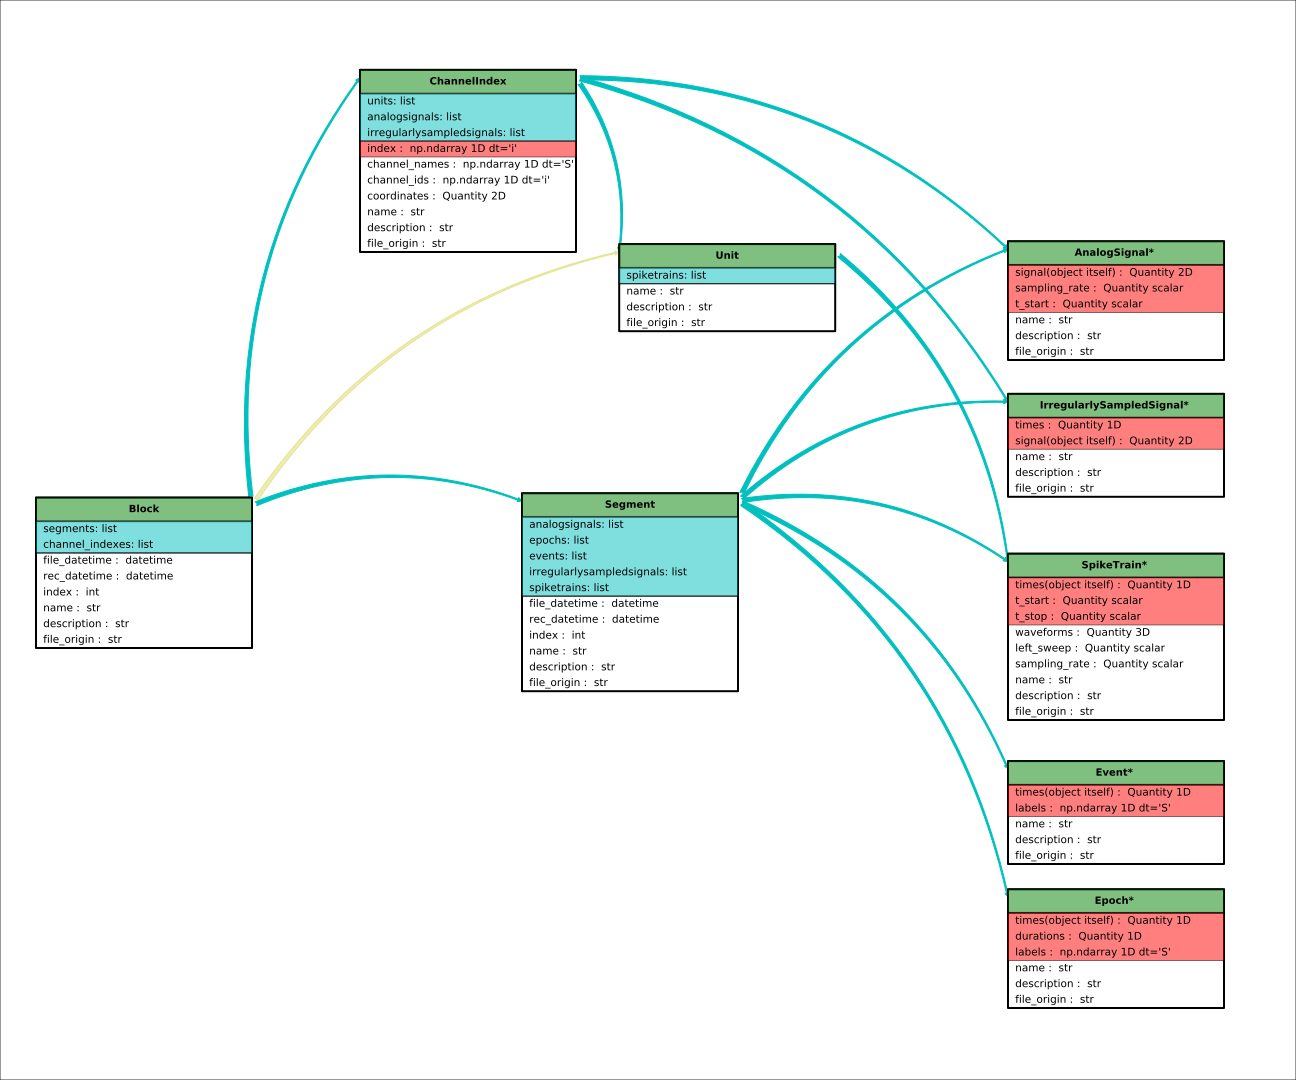
\includegraphics[width=\textwidth]{./Figures/simple_generated_diagram.png}
    \label{fig:neo_uml}
    \caption{Neo 0.7 object structure. Figure modified from \url{https://github.com/neuralensemble/python-neo}.}
\end{figure}


\begin{figure}
    \centering
    \def\svgwidth{\textwidth}
    \input{./Figures/neo_architecture7.tex}
    \label{fig:neo_architecture}
    \caption{Neo 0.7 architecture. Neo represents electrophysiology signals in data objects such as \code{AnalogSignal}s, \code{IrregularlySampledSignal}s and \code{SpikeTrain}s optionally including information about waveform data for each spike. Additional supplementary information describing the timing during the recording can be provided using \code{Event}s or \code{Epoch}s to mark time points or durations during the recording, respectively. All above described data objects are put into relation by container objects, such as \code{Segment}s (grouping all data objects simultaneous in time), \code{Unit}s (grouping \code{SpikeTrain}s across time) and \code{ChannelIndex}es (grouping \code{AnalogSignal}s \code{IrregularlySampledSignal}s and \code{Unit}s). The top level container is a \code{Block} linking to \code{Segment}s and \code{ChannelIndex}es. Figure modified from \url{https://github.com/neuralensemble/python-neo}.}
\end{figure}


% ...
% \subsection{Exemplary Figure}
% \label{subsec:Section_Name/fig}
% ...
% \begin{figure}[htbp]
%     \centering
%     \includegraphics[width=.5\linewidth]{./Figures/UoC_Logo.png}
%     \caption{Exemplary Figure}
%     \label{fig:UoC}
% \end{figure}
% 
% 
% \subsection{Exemplary Figure Referencing}
% \label{subsec:Section_Name/fig_rfs}
% 
% See Figure \ref{fig:UoC} for details. Additional information can be
% found in the footnote \footnote{Image taken from \url{https://en.wikipedia.org/wiki/File:Siegel_Uni-Koeln_(Grau).svg}.}.
